\documentclass[english,t,aspectratio=169,xcolor=table,usenames,dvipsnames]{beamer} %1610, 149, 54, 43 and 32.
%%%%
%%%Title page%%%%%%%%
\title[What is a Proof? ...What is Math?]{What is a Proof? ...What is Math?}
\subtitle{A "fun" introduction to the maths you didn't know you loved.}
\author{Dr.\. Jim Ashe}
\titlegraphic{\vspace{-15pt}
\includegraphics[height=2.25cm]{pics_shared/WGU_logo.png}}
\institute{IT College \\Mathematics, Computer Science, Data Analytics, \textbf{Capstone}}
%preamble{
\usepackage{beamer-JA}
\usepackage{tikz,calc}
\usetikzlibrary{calc,positioning,arrows,arrows.meta,shapes, shapes.geometric,fit}
\usepackage{adjustbox}
\usepackage{wasysym} %for symbols
% \usepackage{venndiagram}
\usepackage{caption}
%\usepackage{booktabs}
%\usepackage{caption,subcaption}
\usepackage{amssymb}
\usepackage{mathtools}

\DeclareMathAlphabet{\mathcal}{OMS}{cmsy}{m}{n}
\SetMathAlphabet{\mathcal}{bold}{OMS}{cmsy}{b}{n} %for big-O
% \setbeamertemplate{footline}[page number] %for coding
% \setbeamertemplate{footline}[totalframenumber]
% \beamerdefaultoverlayspecification{<+->}
\newcounter{num}
\setcounter{num}{1}
\newcounter{numTemp}
\setcounter{numTemp}{1}
%%%%Chapter and Section numbers%%%%% 
% \newcommand{\chNum}{}
% \newcommand{\secNum}{}
\newcommand{\secTitle}{C964 section title}
\date{}
%\date{\formatdate{29}{9}{2015}}

%tikz settings{
%}
\definecolor{blueWGU}{RGB}{0,48,87}
\definecolor{lightBlueWGU}{RGB}{73,134,160}

\definecolor{uablue}{RGB}{0,61,100}
\colorlet{uablue100}{uablue}
\colorlet{uablue75} {uablue!75!white}
\colorlet{uablue50} {uablue!50!white}
\colorlet{uablue25} {uablue!25!white}
\colorlet{uablue10} {uablue!10!white}
\colorlet{uablue5}  {uablue!5!white}

\definecolor{uared}{RGB}{126,0,47}
\colorlet{uared100}{uared}
\colorlet{uared75} {uared!75!white}
\colorlet{uared50} {uared!50!white}
\colorlet{uared25} {uared!25!white}
\colorlet{uared10} {uared!10!white}
\colorlet{uared5}  {uared!5!white}

\tikzset{onslide/.code args={<#1>#2}{%
  \only<#1>{\pgfkeysalso{#2}} % \pgfkeysalso doesn't change the path
}}
\tikzset{alt/.code args={<#1>#2#3}{%
  \alt<#1>{\pgfkeysalso{#2}}{\pgfkeysalso{#3}} % \pgfkeysalso doesn't change the path
}}
\tikzset{temporal/.code args={<#1>#2#3#4}{%
  \temporal<#1>{\pgfkeysalso{#2}}{\pgfkeysalso{#3}}{\pgfkeysalso{#4}} % \pgfkeysalso doesn't change the path
}}
%for fancy arrows
\tikzset{
node distance = 9em and 4em,
%sloped,
   box/.style = {%
    shape=rectangle,
    rounded corners,
    draw=blue!40,
    fill=blue!15,
    align=center,
    font=\fontsize{12}{12}\selectfont},
    double -latex/.style args={#1 colored by #2 and #3}{
        -latex,line width=#1,#2,
        postaction={draw,-latex,#3,line width=(#1)/3,shorten <=(#1)/4,shorten >=4.5*(#1)/3},
    },
    arrow/.style args= {#1}{%
        draw=black,
        line width=2mm,% <-- select desired width
        -{Triangle[length=3.25mm]},
        shorten >=1mm, shorten <=1mm,
        font=\fontsize{8}{8}\selectfont,
        postaction={draw=#1!35,line width=1.75mm,-{Triangle[length=2.75mm]},shorten >=1.25mm,shorten <=1.25mm}
        },
    arrow/.default={blue} %arrow2/.default={blue}{yellow}
}

\tikzstyle{block} = [rectangle, draw, fill=uablue25,
    text width=4.5em, text centered, rounded corners, minimum height=3.25em, line width=1pt ]
\tikzstyle{block2} = [rectangle, draw, fill=uablue25,
    text width=3.0em, text centered, rounded corners, minimum height=4.0em, line width=1pt ]
\tikzstyle{block3} = [rectangle, rounded corners, line width = 1pt, draw, fill=uablue25, text centered, minimum width=6em, minimum height = 2em, inner sep =0em]

\tikzstyle{mysquare} =[rectangle, draw, text width=4em, text centered, rounded corners, minimum height=2cm, minimum width=2cm, line width=2pt,fill=red!50!white]
\tikzstyle{mydiamond} =[diamond, draw, text width=4em, text centered, rounded corners, minimum height=2cm, minimum width=2cm, line width=2pt,fill=blue!50!white]
\tikzstyle{mycircle} =[circle, draw, text width=4em, rounded corners, line width=2pt]
%\tikzstyle{subsetset} = [thick,aspect=0.7,minimum height=1.7cm,minimum
%                            width=1.5cm, align = center]
\tikzstyle{cylinderl} = [
    minimum width=1.5 cm, minimum height=1.75 cm,
    inner sep=0pt,
    align=center]

% cylinder node
\tikzset{
  pics/myCylinder/.style args = {#1}{ %#1/#2/#3.. for multiple args
    code = {
%    \pgfsize{\mywidth}{\myheight} %can use \mywidth to direcly get box value
    \node[name=origin] at (0,0) { }; %places one box corner at 0,0
    \useasboundingbox (origin);
    \def\cTop{.2}; %1cm = 28.3464567 pt
%    \coordinate (UR) at (\mywidth/2,\myheight/2-\cTop);
    \coordinate[below=\cTop of current bounding box.north east] (UR);
    \coordinate[above=\cTop of current bounding box.south east] (LR);
    \coordinate[above=\cTop of current bounding box.south west] (LL); %correct
    \coordinate[below=\cTop of current bounding box.north west] (UL);
    \coordinate[below=\cTop of current bounding box.north] (top);

%    \draw[thick, green] let \p1 = (UR), \p2 = (UL) in (\x1-\x2,0) -- (LR) -- (LL) -- (UL) -- cycle;
    \draw[fill = #1,draw] let \p1 =(UR), \p2 = (UL) in (LL) arc[start angle=180, end angle = 360, radius =\x1/2-\x2/2, y radius = \cTop cm] -- (UR) -- (UL) -- (LL) -- cycle;
    \draw [fill =#1!75!black] let \p1 =(UR), \p2 = (UL) in (top) ellipse (\x1/2-\x2/2 and \cTop cm); %top
    \draw (LL)--(UL); %left
    \draw (UR)--(LR); %right
    \draw let \p1 =(UR), \p2 = (UL) in (LL) arc (180:360:\x1/2-\x2/2 and \cTop cm); %bottom front base
    \node[font=\Large] at (0,-\cTop/2) {\tikzpictext}; %[block] to see outline for placement
    }
  }
}
\tikzstyle{line} = [line width=1pt, -triangle 45]
\tikzset{
  mycustomnode/.style={
    draw,
    single arrow,
    single arrow head extend=0,
    shape border uses incircle,
    shape border rotate=-90,
  }
}
% \tikzstyle{alert} = [text=uared100, fill=uared25, draw=uared100]
\tikzstyle{dim} = [text=uablue25, fill=uablue5, draw=uablue25]
\tikzstyle{highlight} = [fill=green!50!white, line width =2pt]
\tikzstyle{off} = [text=white, fill=white, draw=white,line width =2pt]
\tikzstyle{dim} = [opacity=.25]
\tikzstyle{myframe} = [line width=4pt, draw=green!65!blue,inner sep=.5em,rounded corners]


% %%for counting slides and frames when debugging
% \newcounter{slidenumber}
% \defbeamertemplate*{footline}{infolines theme frame plus slide}{
%     \setcounter{slidenumber}{\insertpagenumber}%
%     \addtocounter{slidenumber}{-\insertframestartpage}%
%     \addtocounter{slidenumber}{1}%
%     \leavevmode%
%     \hbox{%
%         \begin{beamercolorbox}[wd=\paperwidth,ht=2.25ex,dp=1ex,center]{date in head/foot}%
%           \ifthenelse{\insertframeendpage=\insertframestartpage}{
%             \insertframenumber/ \inserttotalframenumber\hspace*{2ex}}{
%             \insertframenumber(\arabic{slidenumber}{})/\inserttotalframenumber\hspace*{2ex}}
%         \end{beamercolorbox}}%
%         \vskip0pt%
%     }
% \setbeamertemplate{footline}[infolines theme frame plus slide]
\usepackage{xcolor,soul}
% \definecolor{lightblue}{rgb}{.90,.95,1}
\sethlcolor{green}
\renewcommand<>{\hl}[1]{\only#2{\beameroriginal{\hl}}{#1}}

%%higlighting tex wiht overlays
\makeatletter
\newcommand\SoulColor{%
  \let\set@color\beamerorig@set@color
  \let\reset@color\beamerorig@reset@color}
\makeatother
\SoulColor
%}

%%%%
\begin{document}
\makebeamertitle 
\nonfrenchspacing %%babel package uses french spacing
%%%input parts
% %%%%%%%%%%
\begin{frame}
    \centering
    \only<1>{%
        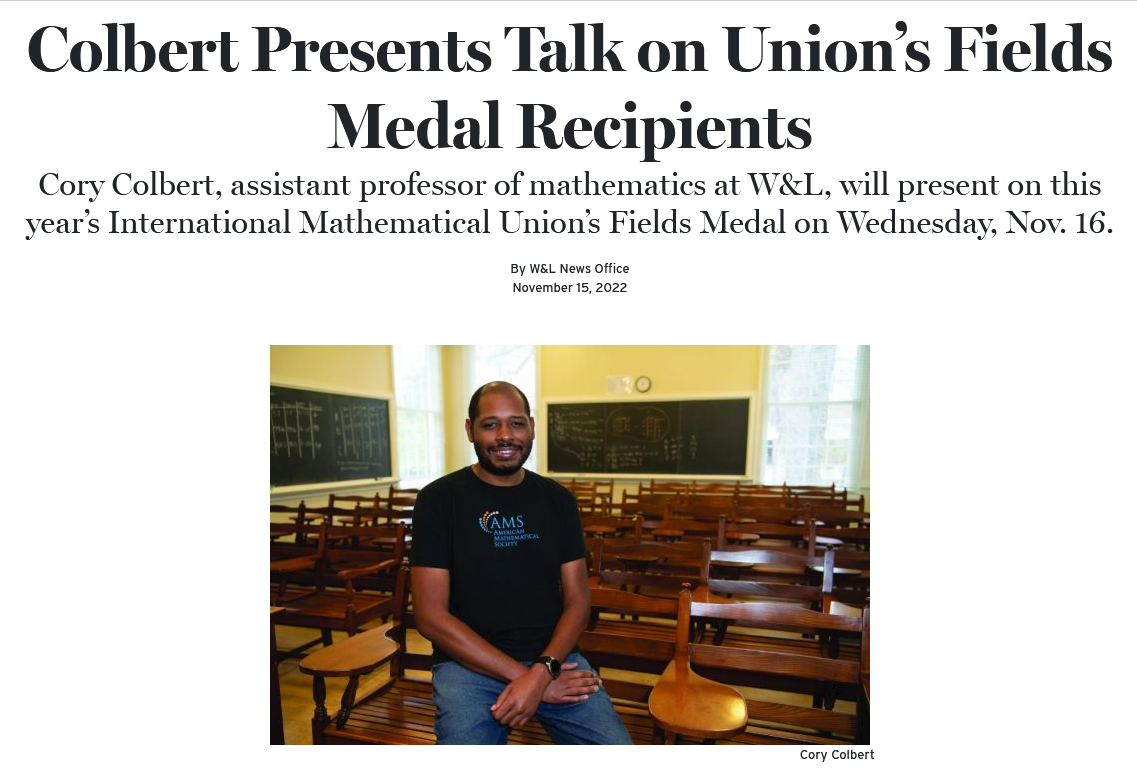
\includegraphics[width=0.85\textwidth]{./images_women_in_IT/colbert_math.png}
        % \caption{This is an example caption.}
    }
    \only<2>{%
        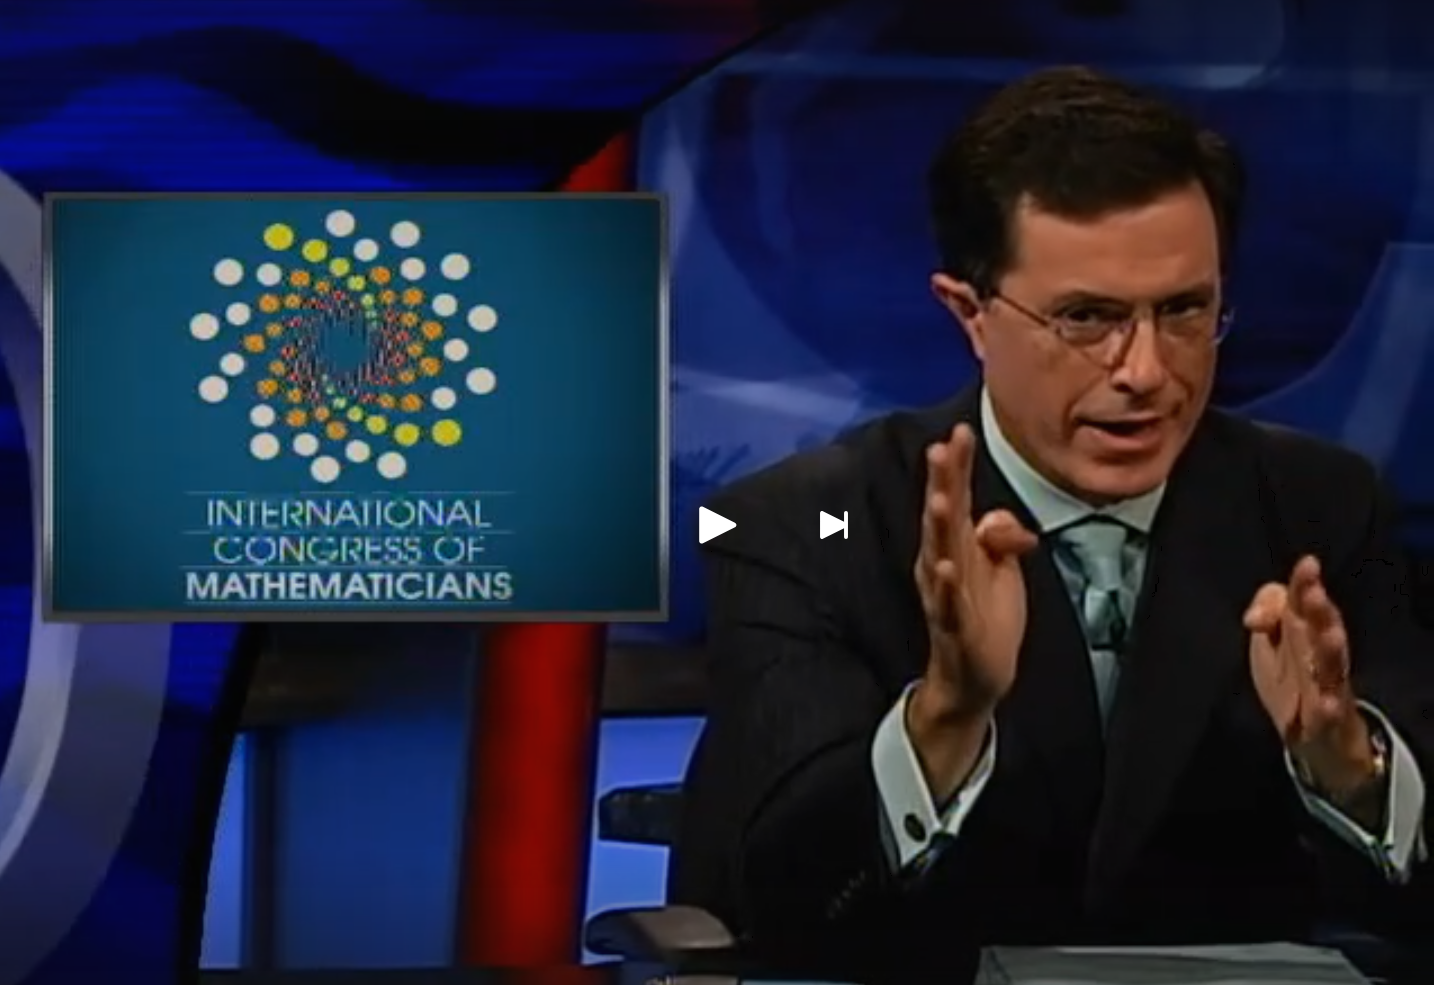
\includegraphics[width=0.75\textwidth]{./images_women_in_IT/stephen_colbert.png}
        \\ \href{https://www.dailymotion.com/video/x7yrghr}{Colbert on the Fields Medal.}
    }
\end{frame}

\begin{frame}{}
    \begin{columns}
        \begin{column}{.65\textwidth}
            \Huge \textbf{What is this stuff?}
            \begin{itemize}
                \item<2->Proof? 
                \item<3->Conjecture?
                \item<4->Weird Stuff with a bunny?
            \end{itemize}
        \end{column}
    \end{columns}
\end{frame}

\begin{frame}
    \centering
    \vfill
    \tikzset{%
        node/.style={draw, align=center, minimum width=2.5cm, minimum height=1cm, text width =2.5cm},
        circ/.style={node, circle, minimum height=1.2cm, text width =2.5cm},
        oval/.style={node, ellipse, minimum height=1.2cm, text width =2.5cm},
        >={Latex[length=3mm]},
        arrow/.style={->, thick}
    }

    \begin{tikzpicture}[scale=.5,node distance=1.6cm]
        % Nodes
        \node[oval, fill=blue!25]   (start) {\small Spot patterns, connect ideas, explore, ...};
        \node[circ, fill=red!25, right=of start, visible on=<2->] (a) {\small Define, structure, abstract, conjecture, ...};
        \node[oval, fill=green!25, right=of a, visible on=<3->] (b) {\small Formalize, communicate, share, ...};
        \node[circ, fill=yellow!75, below =1cm of a, visible on=<4->] (d) {Understand\\ (hard things)};
        \node[circ, fill=yellow!60!red, below= of start, visible on=<7->] (end) {\small "Real-world"\\ tools};

        % Arrows
        \draw<2->[arrow] (start) -- (a);
        \draw<3->[arrow] (a) -- (b);
        \draw<4->[arrow] (b) |- (d);
        \draw<5>[arrow] (d) -| (start);
        \draw<7>[arrow] (d) -- (end);
        \draw<7>[arrow] (end) -- (start);
    \end{tikzpicture}
    \onslide<6->{The language of this process is "proof," and logic is its grammar.}
    \vfill
\end{frame}

\begin{frame}
    \only<1>{%
        \centering
        \vfill
        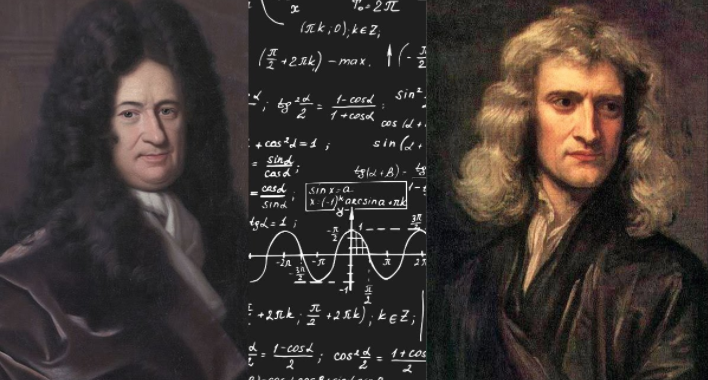
\includegraphics[width=0.85\textwidth]{./images_women_in_IT/newton_leibniz_calculus.png}
        % \caption{This is an example caption.}
    }
    \only<2->{%
            \vfill
            \textit{“I have never done anything ‘useful’. 
            No discovery of mine has made, or is likely to make, directly or indirectly, for good or ill, 
            the least difference to the amenity of the world.”} \\
            \hfill -G. H. Hardy (number theory) 1877–1947
    }
    \\ \vspace{30pt}
    \only<3->{%
            \textit{“Vector analysis is interesting, but it will never have any practical application.”}\\
            \hfill -William Thomson (Lord Kelvin) 1824-1907
    }
    \vfill
\end{frame}
\input{part_1b.tex}

%%pyramid%%%
\begin{frame}{}
    \Large
    \centering
    The langauge of maths is \textbf{proof}.\\ 
    \normalsize 
    % \vspace{10pt}
    \begin{columns}
        \textbf{\null}%place holder
        \begin{column}{.5\textwidth}
            \only<2-3,10->{%
                \begin{itemize}
                    \item<2->[] But what is a proof???
                    \item<10->[] A way to communicate aboslute tRUTHS, through logic.
                \end{itemize}
            %     \begin{itemize}
            % %         
            %     \end{itemize}
            }
            \vspace{20pt}
            \Large \only<11->{If (something is true)}
            \only<12->{then (something else is true)}
        \centering 
            \only<4>{\begin{figure}
                \centering
                \includegraphics[width =.6\textwidth]{./images_women_in_IT/Georg_Cantor_eyes_smile.png}
                \caption*{Georg Cantor (1845-1918)}
            \end{figure}}
            \only<5>{\begin{figure}
                \centering
                \vspace{20pt}
                \includegraphics[width =.6\textwidth]{./images_women_in_IT/Boole.png}
                \caption*{George Boole (1815-1864)}
            \end{figure}}
            \only<6-9>{\begin{figure}
                \centering
                \vspace{20pt}
                \includegraphics[width =.6\textwidth]{./images_women_in_IT/BooleCool.png}
                \caption*{George Boole (1815-1864)}
            \end{figure}}
        \end{column}
        
        %%%%
        \begin{column}{.5\textwidth}
            \vspace{10pt}
            \begin{figure}
                \includegraphics<3>[width=.8\textwidth]{./images_women_in_IT/mathpyramid1.png}
                \includegraphics<4>[width=.8\textwidth]{./images_women_in_IT/mathpyramid2.png}
                \includegraphics<5>[width=.8\textwidth]{./images_women_in_IT/mathpyramid3.png}
                \includegraphics<6>[width=.8\textwidth]{./images_women_in_IT/mathpyramid4.png}
                \includegraphics<7>[width=.8\textwidth]{./images_women_in_IT/binary.png}
                \includegraphics<8>[width=.8\textwidth]{./images_women_in_IT/graphs.png}
                \includegraphics<9-12>[width=.8\textwidth]{./images_women_in_IT/binary.png}
                \includegraphics<13>[width=.9\textwidth]{./images_women_in_IT/code_example.png}
            \end{figure}    
        \end{column}
    \end{columns}
\end{frame}

\begin{frame}[t]
\frametitle{You've all dones this.} 
\large
    \[
        \begin{array}{rcl}
            \onslide<2->{x^2 -2x-15 &=& 0} \\[6pt]
            \onslide<3->{x^2 -5x + 3x -15 &=& 0} \\[6pt]
            \onslide<4->{(x-5)(x+3)&=& 0} \\[6pt]
            \onslide<5->{x&=& 5 \text{ or } -3 } 
        \end{array}
    \]
\end{frame}

\begin{frame}[t]
    \vfill
    \begin{columns}
        \begin{column}{.35\textwidth}
            \begin{itemize}
                \item<2-> Direct proof. 
                \item<3-> Proof by contradiction.
                \item<4-> Proof by induction. 
            \end{itemize}
        \end{column}
        %%%%
        % \begin{column}{.55\textwidth}
        % \end{column}
    \end{columns}
    \vspace{20pt}
    % \centering
    % \only<3>{If \textbf{A} then \textbf{B}}
    % \only<5>{If (\textbf{A} then \textbf{NOT B}), then something absurd, then If \textbf{A} then \textbf{B}}
    % \only<7>{If \textbf{A} for $n$ then \textbf{A} $n+1$, and \textbf{A} for some $n=x$, then \textbf{A} for all $n\geq X$.}
\end{frame}

% \begin{frame}[t]
% \frametitle{You've all dones this.}
% A phone, a phone, and a phone are added to an unknown number of phones. The result is equal to a phone, phone, phone, phone, and phone. 
% \\ \vspace{20pt}
% \Large
% \centering
% \only<2>{\phone, \phone, \& \phone{} are  added to an \framebox{? \phone's}. The result is equal to \phone, \phone, \phone, \phone, \& \phone. }
% \only<3>{$3 \times$ \phone's are  added to an \framebox{? \phone's}. \\The result is equal to $5 \times$ \phone's. }
% \only<4>{$3 \times $ \phone's $+$ \framebox{? \phone's} $ = 5 \times $\phone's. }
% \only<5>{$3  +$ \framebox{? \phone's} $ = 5$. }
% \only<6->{$3 + x = 5$}
% \vspace{10pt}
% \only<7>{\\ $\Rightarrow x = 8$ }
% \only<8>{\\ $\Rightarrow x = 2$ }
% \normalsize
% \end{frame}
%%%%hand and sets
\begin{frame}{}
    \begin{columns}
        \begin{column}{\textwidth}
            \centering
                \adjustbox{max width =\textwidth, min height=9cm}{%
                \begin{tikzpicture}
                    %hand
                    \visible<-7>{\node [above right,inner sep=0] (hand) at (0,0) {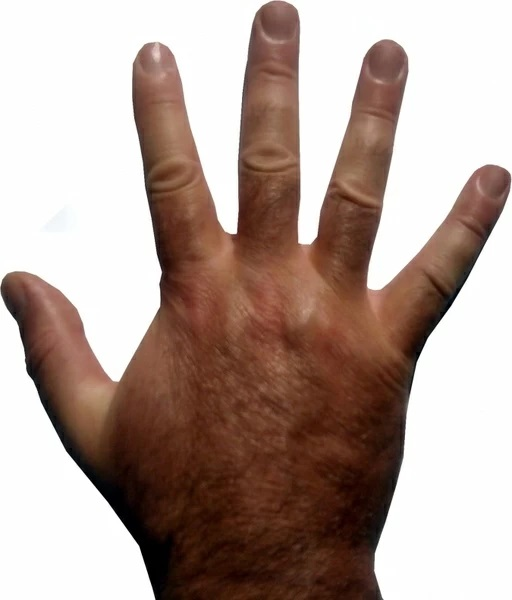
\includegraphics[width=3cm]{./images_5-20-2022/hand5.png}};}
                    
                    \node [above = .5cm of hand] (set) {{\visible<8->{\{}}\sun {\visible<8->{,}} \phone{\visible<8->{,}} \smiley{\visible<8->{,}} \twonotes{\visible<8->{,}} {\visible<7->{\frownie}}{\visible<8->{\}}} };
                          
                    \node<9-> [below = .5cm of set] (set2) {\{1, 2, 3, 4, 5\}};
                    % \draw[above right,help lines,step=5mm,gray!20] (0,0) grid (3,5);
                    
                    %thumb
                    \draw<2-7>[latex-, very thick, Green] (.5, 4.25) -- (.25, 1.95);
                    %index
                    \draw<3-7>[latex-, very thick, Green] (1.0, 4.25) -- (.9, 3.325);
                    %middle
                    \draw<4-7>[latex-, very thick, Green] (1.6, 4.25) -- (1.6125, 3.55);
                    %ring
                    \draw<5-7>[latex-, very thick, Green] (2.1, 4.25) -- (2.25, 3.325);
                    %pinky
                    \draw<6>[latex-, very thick, red] (2.58, 4.25) -- (2.85, 2.6) 
                    node[above, pos=0.1,red]{X};
                    \draw<7>[latex-, very thick, Green] (2.58, 4.25) -- (2.85, 2.6) ;
                    
                    %set arrows
                    \draw<9->[latex-, very thick, Green] (.5, 4.25) -- (.6, 3.45);
                    %index
                    \draw<9->[latex-, very thick, Green] (1.0, 4.25) -- (1.05, 3.45);
                    %middle
                    \draw<9->[latex-, very thick, Green] (1.6, 4.25) -- (1.5, 3.45);
                    %ring
                    \draw<9->[latex-, very thick, Green] (2.1, 4.25) -- (1.95, 3.45);
                    %pinky
                    \draw<9->[latex-, very thick, Green] (2.58, 4.25) -- (2.35, 3.45); 
                    
                    \node<10-> [below = .5cm of set2] (set3) {\{5, 4, 3, 5\}\textcolor{white}{, 1}};
                    
                    \draw<11->[-latex, very thick, Green] (.65, 3) -- (.65, 2.25);
                    %index
                    \draw<11->[-latex, very thick, Green] (1.05, 3) -- (1.05, 2.25);
                    %middle
                    \draw<11->[-latex, very thick, Green] (1.5, 3) -- (1.5, 2.25);
                    %ring
                    \draw<11->[-latex, very thick, Green] (1.95, 3) -- (1.95, 2.25);
                    %pinky
                    \draw<11->[-latex, very thick, red] (2.35, 3) -- (2.35, 2.25) node[below, pos=0.85,red]{X};
                    
                    \node<-7> [align =center ] at (-1.5,3) {More fingers \\or symbols?};
                    \node<12-> [below = .1cm of set3, align = center] {\tiny "The essence of math is not to make simple things complicated,\\ \tiny but to make \textit{complicated things simple}."};
                \end{tikzpicture}
                }
        \end{column}
    \end{columns}
\end{frame}

%%%hilbert hotel%%%
\begin{frame}{}
    % \Large \textbf{What is Math(s)?}
    % \normal
    % \null \vfill
    \colorlet{soulred}{red!25}
    \colorlet{soulgreen}{green!25}
    \begin{columns}
        \begin{column}{.43\textwidth}
             \uncover<3->{\textbf{Are these two sets the same?}} 
             \\ \uncover<4->{\hspace{.5cm} No.} 
             \\ \uncover<5->{\textbf{Are these two sets the same \textit{size}?}}
             \\ \uncover<16->{\hspace{.5cm} Yes!}
             \begin{itemize}
                 \item<2->[]\sethlcolor{soulred}\hl<2>{$\mathbb{N} = \{1, 2, 3, 4, \dots\}$}
                 \item<3->[]\sethlcolor{soulgreen}\hl<3>{$\mathbb{N}_{0} = \{0, 1, 2, 3, 4, \dots\}$} 
             \end{itemize}
                %%%%%%venn diagram
                \vspace{6pt}
                \begin{tikzpicture}[scale=1.0, envel/.style={shape=ellipse, draw, inner sep=-0.5cm}]
                	\def\circleA{(1.4,0) circle (1)} 
                	%\node[anchor=south] at (current bounding box.north) {$A \cap B$}; 
                    \large
                    \node (1) at (1.5,.5) {$1$};
                    \node (2) at (1.65,-.5) {$2$};
                    \node (3) at (1.25,.75) {$3$};
                    \node (4) at (.6,-.1) {$4$};
                    \node (0) at (0,0) {$0$};
                    \node (-5) at (-1.5,.65) {$-5$};
                    \node (sqrt) at (3.25,.25) {$\sqrt{2}$};
                    \node (pi) at (3.5,-1) {$\pi$};
                    \node (frac1) at (-1.6,-1.125) {$-\frac{1}{2}$};
                    \node (frac2) at (2.8,1) {$\frac{5}{3}$};
                	\node<3->[draw, thick, fill = green!35, inner sep=.15cm, fit=(1)(2)(3)(0),shape=ellipse] (gc) { };
                	\draw<2->[draw, thick, fill = red!35] \circleA node {\dots }; 
                    \foreach \n in {0,1,2,3,4} {%
            	        \node at (\n) {$\n$};
                	}   
                    % \node (a) at (1.25,4.25) {$2$};
                	\draw[very thick] (-2,-2) rectangle (4,2) node[anchor=north west] at (current bounding box.north west) {$\mathbb{R}$}; 
                \end{tikzpicture}
                %%%%%%%%%%%%
        \end{column}
        \only<6->{%
        \begin{column}{.5\textwidth}
            \textbf{The Hilbert Hotel Problem}
            % \vspace{12pt}
            \only<7>{%
                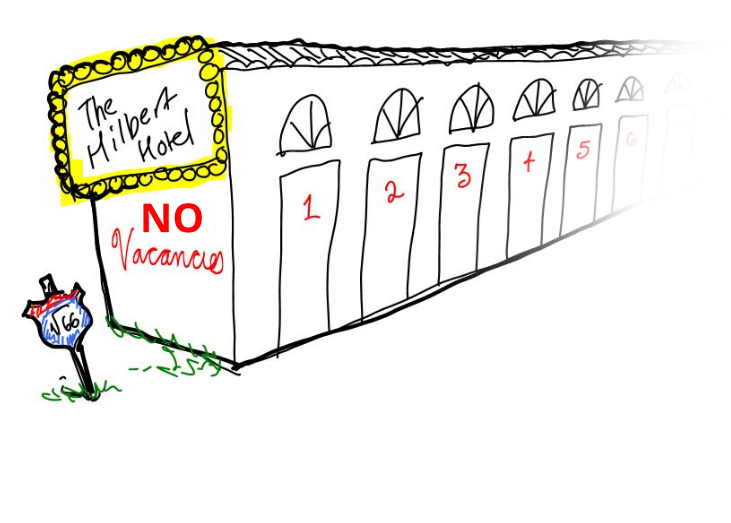
\includegraphics[width =\textwidth]{./images_5-20-2022/hilbert_hotel0.png}
            }
            \only<8>{%
                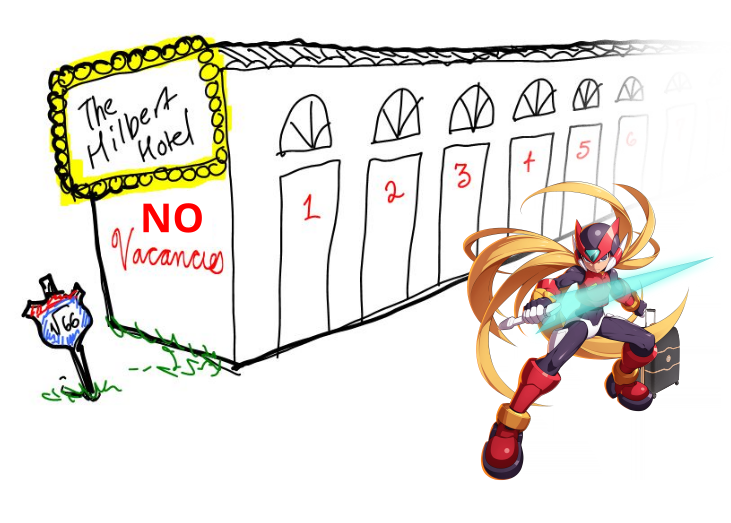
\includegraphics[width =\textwidth]{./images_5-20-2022/hilbert_hotel1.png}
                }
            \only<9>{%
                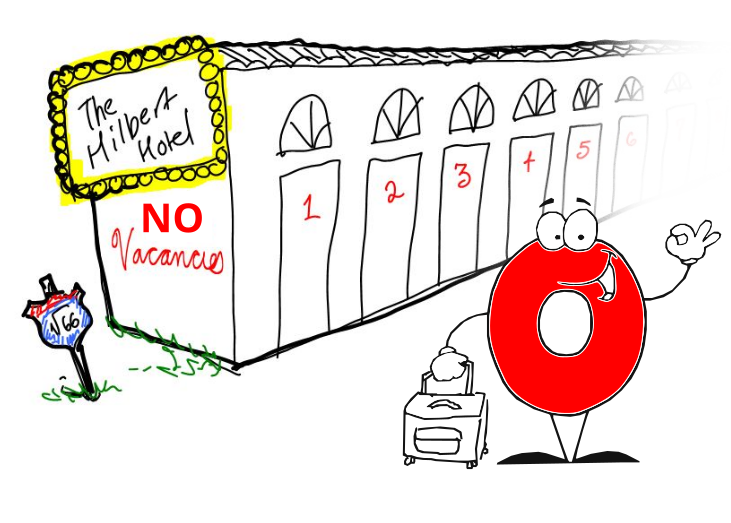
\includegraphics[width =\textwidth]{./images_5-20-2022/hilbert_hotel2.png}
            }
            \only<10>{%
            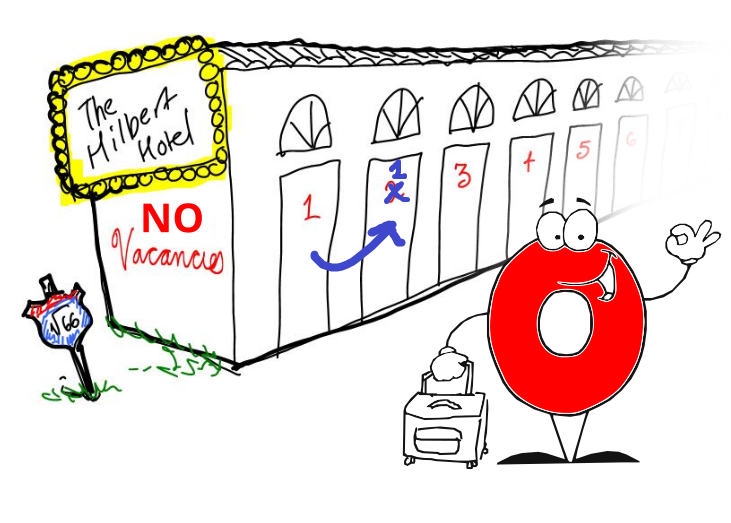
\includegraphics[width =\textwidth]{./images_5-20-2022/hilbert_hotel3.png}}
            \only<11>{%
            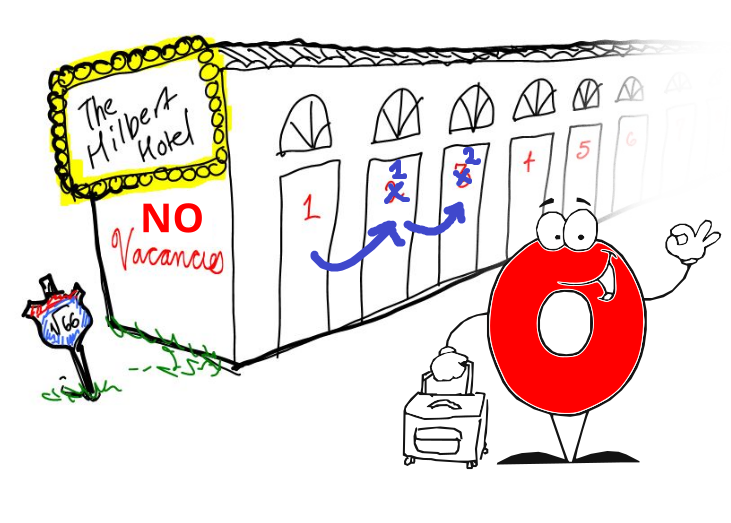
\includegraphics[width =\textwidth]{./images_5-20-2022/hilbert_hotel4.png}}
            \only<12>{%
            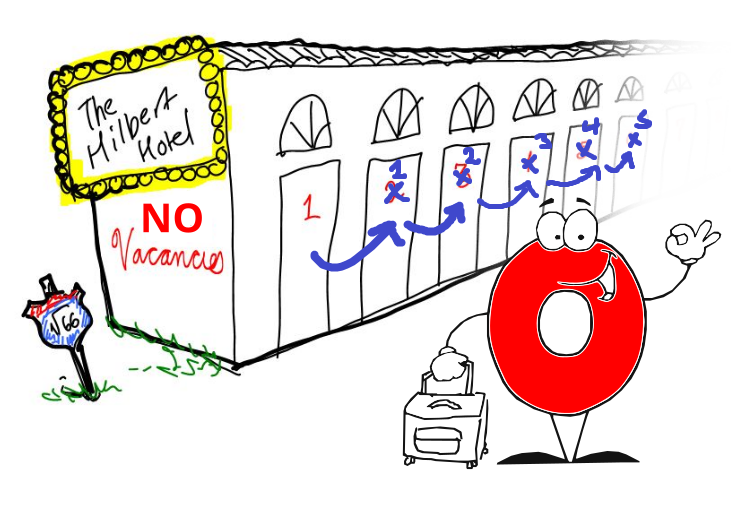
\includegraphics[width =\textwidth]{./images_5-20-2022/hilbert_hotel5.png}}
            \only<13>{%
            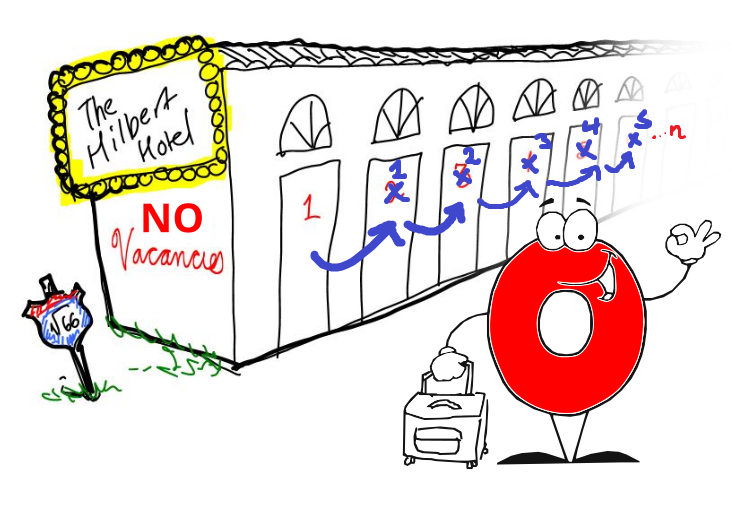
\includegraphics[width =\textwidth]{./images_5-20-2022/hilbert_hotel6.png}}
            \only<14>{%
            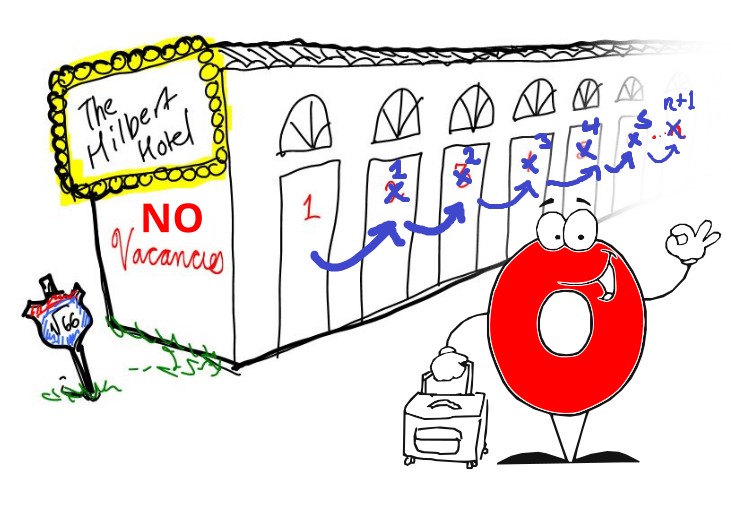
\includegraphics[width =\textwidth]{./images_5-20-2022/hilbert_hotel7.png}}
            \only<15->{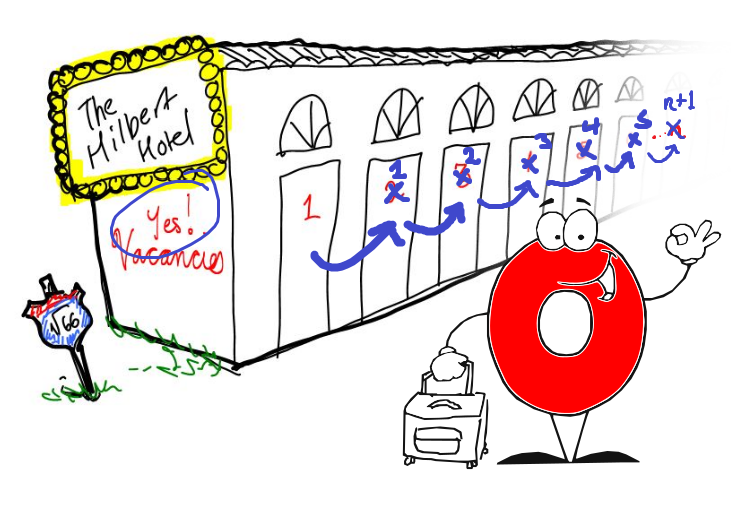
\includegraphics[width =\textwidth]{./images_5-20-2022/hilbert_hotel8.png}}
            \\ \only<17->{We call these sets \textit{countable}} 
            \only<18->{\dots because we can \textit{count} them.}
        \end{column}
        }
    \end{columns}
    % \vfill
\end{frame}

% rational numbers countable
\begin{frame}{}
    \begin{columns}
        \colorlet{soulblue}{blue!25}
        \colorlet{soulred}{red!25}
        \begin{column}{.43\textwidth}
             \textbf{Are these two sets the same size?}
             \\ \uncover<33->{\hspace{.5cm} Yes!}
             \begin{itemize}
                 \item<1->[]\sethlcolor{soulred}\hl<1>{$\mathbb{N} = \{1, 2, 3, 4, \dots\}$}
                 \item<2->[]\sethlcolor{soulblue}\hl<2>{$\mathbb{Q} = \{\frac{1}{2}, \frac{3}{4}, \frac{5}{3}, -1, 4, 0,\dots\}$} 
             \end{itemize}
                %%%%%%venn diagram
                \vspace{6pt}
                \begin{tikzpicture}[scale=1.0, envel/.style={shape=ellipse, draw, inner sep=-0.5cm}]
                	\def\circleA{(1.4,0) circle (1)} 
                    \large
                	%nodes must be defined previously
                	\node<2->[draw,fill = blue!25, inner sep=.5ex, rounded corners =.7cm, thick, fit=(frac1) (frac2)] { };
                	\draw[draw, thick, fill = red!35] \circleA node {\dots }; 
                	
                    \node (1) at (1.5,.5) {$1$};
                    \node (2) at (1.65,-.5) {$2$};
                    \node (3) at (1.25,.75) {$3$};
                    \node (4) at (.6,-.1) {$4$};
                    \node (0) at (0,0) {$0$};
                    \node (-5) at (-1.5,.65) {$-5$};
                    \node (sqrt) at (3.25,.25) {$\sqrt{2}$};
                    \node (pi) at (3.5,-1) {$\pi$};
                    \node (frac1) at (-1.6,-1.125) {$-\frac{1}{2}$};
                    \node (frac2) at (2.8,1) {$\frac{5}{3}$};
                	\draw[very thick] (-2.25,-2) rectangle (4,2) node[anchor=north west] at (current bounding box.north west) {$\mathbb{R}$}; 
                \end{tikzpicture}
                \centering
                \vspace{-10pt}
                
                \begin{tikzpicture}[scale=2.0]
                    \node<3->[above,white] at (.5,0) {$\frac{1}{2}$};
                    \draw<3->[latex-latex] (-.5,0) -- (1.5,0) ; %edit here for the axis
                	\foreach \x in  {0,1} 
                        \draw<3->[shift={(\x,0)},color=black] (0pt,2pt) -- (0pt,-2pt);
                	\foreach \x in  {0,1} 
                        \draw<3->[shift={(\x,0)},color=black] (0pt,0pt) -- (0pt,-3pt) node[below] {$\x$};
                    \node<4->[above,blue] at (.5,0) {$\frac{1}{2}$};
                        \draw<4->[blue,color=blue,very thick] (.5,1.5pt) -- (.5,-2pt);
                    \node<5->[above,blue] at (.25,0) {$\frac{1}{4}$};
                        \draw<5->[blue,color=blue,very thick] (.25,1.5pt) -- (.25,-2pt);
                    \node<6->[above,blue] at (.125,0) {$\frac{1}{8}$};
                        \draw<6->[blue,color=blue,very thick] (.125,1.5pt) -- (.125,-2pt);
                    \foreach \x in {16,32,64,128,256}
                        \draw<7->[blue,color=blue,very thick] ({1/\x},1.5pt) -- ({1/\x},-2pt);
                    \node<8->[above,blue] at (0.0001,0) {$\frac{1}{\infty}$};
                \end{tikzpicture}
                
                %%%%%%%%%%%%
        \end{column}
        %%%%%
        \only<9->{%
        \begin{column}{.5\textwidth}
            \vspace{15pt}
            \only<10>{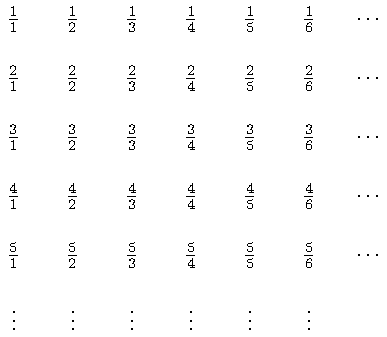
\includegraphics[width =\textwidth]{./images_5-20-2022/rationalmaps_9.pdf}}
            \only<11>{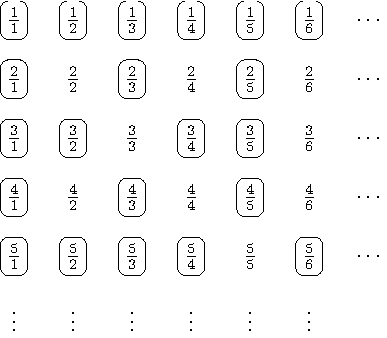
\includegraphics[width =\textwidth]{./images_5-20-2022/rationalmaps_11.pdf}}
            \only<12>{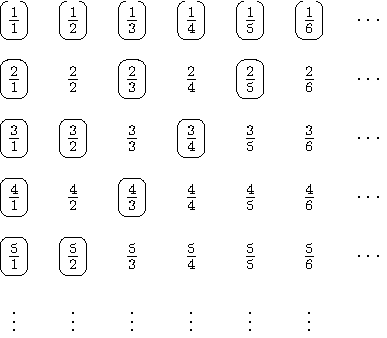
\includegraphics[width =\textwidth]{./images_5-20-2022/rationalmaps_14.pdf}}
            \only<13>{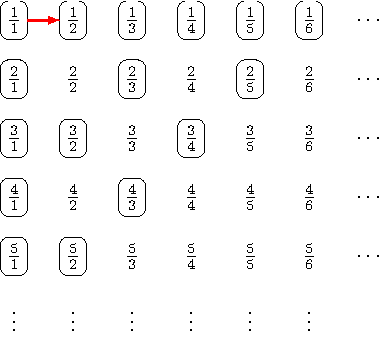
\includegraphics[width =\textwidth]{./images_5-20-2022/rationalmaps_17.pdf}}
            \only<14>{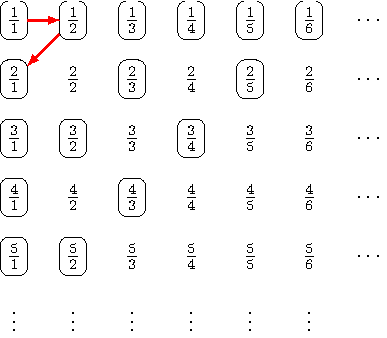
\includegraphics[width =\textwidth]{./images_5-20-2022/rationalmaps_4.pdf}}
            \only<15>{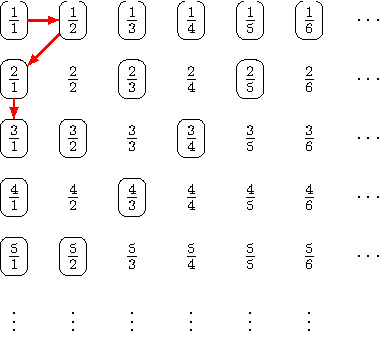
\includegraphics[width =\textwidth]{./images_5-20-2022/rationalmaps_5.pdf}}
            \only<16>{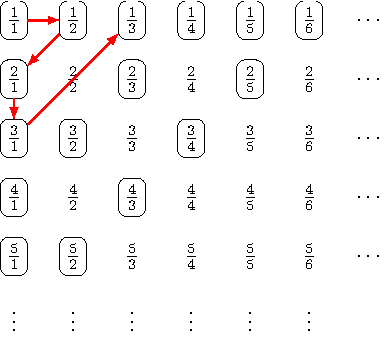
\includegraphics[width =\textwidth]{./images_5-20-2022/rationalmaps_15.pdf}}
            \only<17>{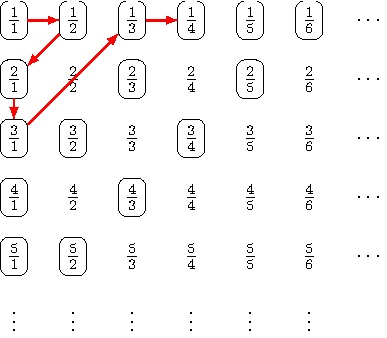
\includegraphics[width =\textwidth]{./images_5-20-2022/rationalmaps_18.pdf}}
            \only<18>{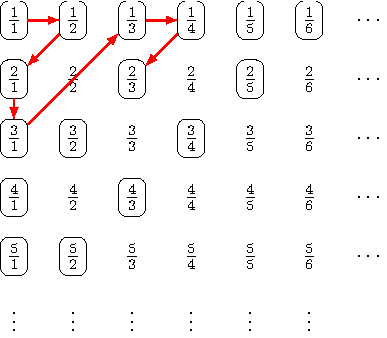
\includegraphics[width =\textwidth]{./images_5-20-2022/rationalmaps_3.pdf}}
            \only<19>{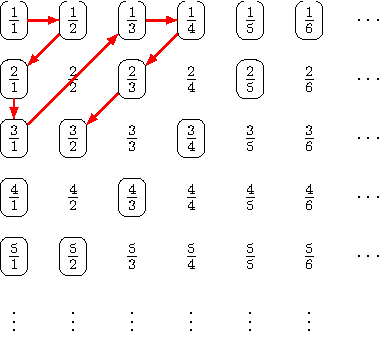
\includegraphics[width =\textwidth]{./images_5-20-2022/rationalmaps_16.pdf}}
            \only<20>{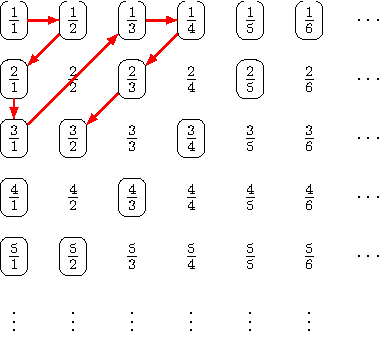
\includegraphics[width =\textwidth]{./images_5-20-2022/rationalmaps_19.pdf}}
            \only<21>{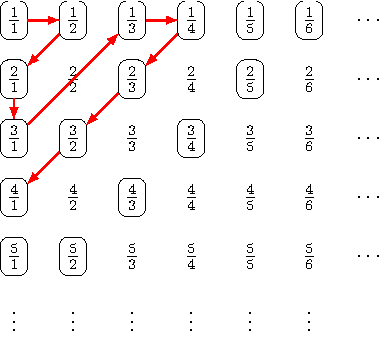
\includegraphics[width =\textwidth]{./images_5-20-2022/rationalmaps_20.pdf}}
            \only<22>{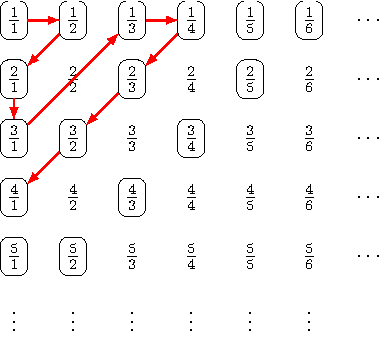
\includegraphics[width =\textwidth]{./images_5-20-2022/rationalmaps_1.pdf}}
            \only<23>{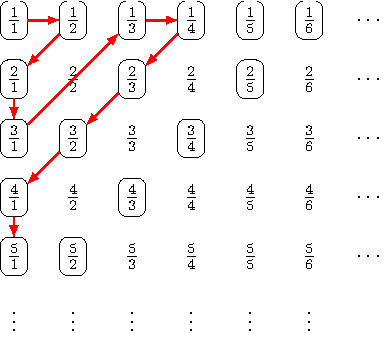
\includegraphics[width =\textwidth]{./images_5-20-2022/rationalmaps_2.pdf}}
            \only<24>{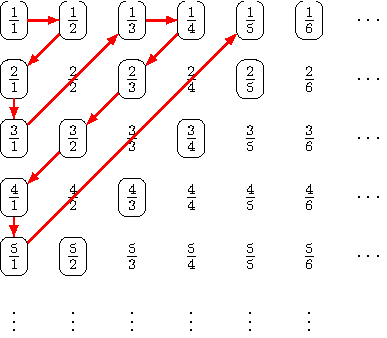
\includegraphics[width =\textwidth]{./images_5-20-2022/rationalmaps_0.pdf}}
            \only<25>{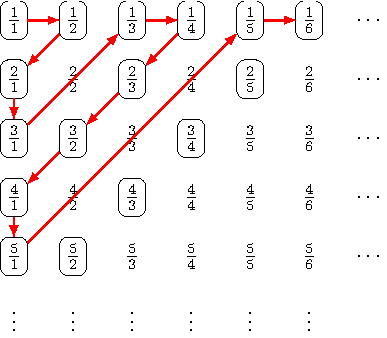
\includegraphics[width =\textwidth]{./images_5-20-2022/rationalmaps_6.pdf}}
            \only<26>{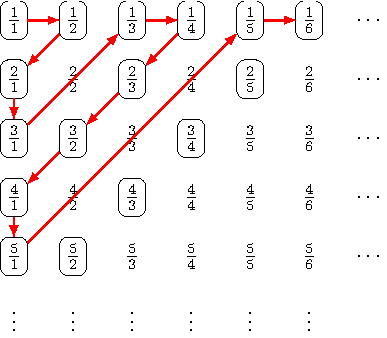
\includegraphics[width =\textwidth]{./images_5-20-2022/rationalmaps_7.pdf}}
            \only<27>{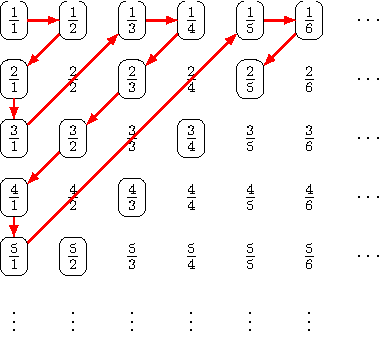
\includegraphics[width =\textwidth]{./images_5-20-2022/rationalmaps_8.pdf}}
            \only<28>{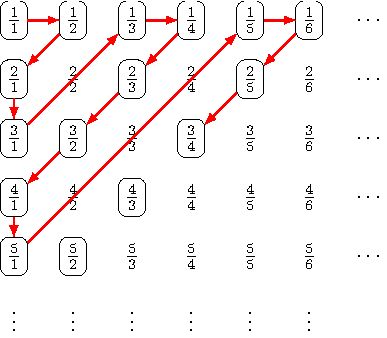
\includegraphics[width =\textwidth]{./images_5-20-2022/rationalmaps_10.pdf}}
            \only<29>{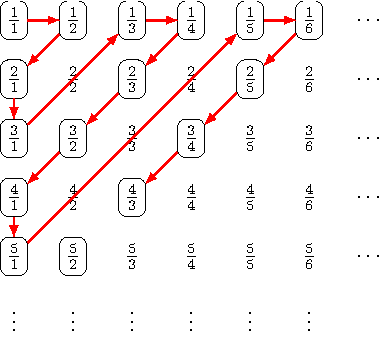
\includegraphics[width =\textwidth]{./images_5-20-2022/rationalmaps_12.pdf}}
            \only<30>{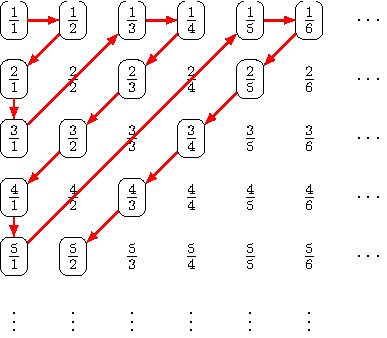
\includegraphics[width =\textwidth]{./images_5-20-2022/rationalmaps_13.pdf}}
            \only<31->{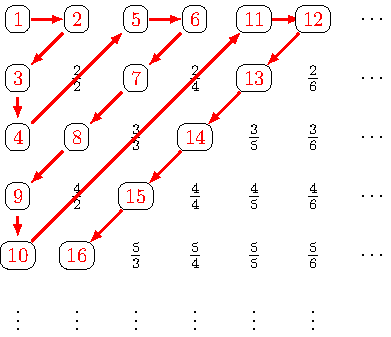
\includegraphics[width =\textwidth]{./images_5-20-2022/rationalmaps_21.pdf}}
            
        \end{column}
        }
    \end{columns}
    % \vfill
\end{frame}

\begin{frame}
    \centering
    \Large
    \vfill
    These are example of "direct" proofs.
    \vfill
\end{frame}


\begin{frame}{}
    \begin{columns}
        \begin{column}{.5\textwidth}
        \textbf{Are all infinite sets the same size?}
        \\\Large 
        \only<2-3>{$|\infty| = |\infty|$?} 
        \only<4-30>{$|\{1, 2, 3, 4, \dots \}| = |\mathbb{R}|$?}
        % \only<12-30>{$|\{1, 2, 3, 4, \dots \}| =$ \normalsize$|\{x\in \mathbb{R}| 0<x<4\}|$?}
        % \normalsize
        \only<31->{No -different infinities!}
            \only<3->{%
                \begin{figure}
                    \centering
                    \includegraphics<3-30>[width =.5\textwidth]{./images_5-20-2022/Georg_Cantor.png}
                    \includegraphics<31>[width =.5\textwidth]{./images_5-20-2022/Georg_Cantor_eyes.png}
                    \includegraphics<32>[width =.5\textwidth]{./images_5-20-2022/Georg_Cantor_eyes_smile.png}
                    \includegraphics<33>[width =.5\textwidth]{./images_5-20-2022/Georg_Cantor_eyes_sad.png}
                    \only<3->{\caption*{Georg Cantor (1845-1918)}}
                    % \icncludegraphics<34>[width =\textwidth]{./images_women_in_IT/HannahCairo-cr.ValeriePlesch-Screen-scaled.png}
                    % \only<34>{\caption*{Mizohata-Takeuchi conjecture\\ Hannah Cairo (2008--)}}
                \end{figure}
                }
        \end{column}
        %%%%
        \begin{column}{.5\textwidth}
            \uncover<5-10>{\textbf{What are the \textit{Real} numbers ($\mathbb{R}$)?}}
            \vspace{10pt}
            
            \only<5-12>{%
                \begin{tikzpicture}[scale=.85]
                    \draw[white] (0,1) circle (1); 
                    \draw[latex-latex] (-1.75,0) -- (5.75,0) ; %edit here for the axis
                        \foreach \x in  {-1,0,1,2,3,4,5} 
                            \draw[shift={(\x,0)},color=black] (0pt,2pt) -- (0pt,-2pt);
                        \foreach \x in {-1,0,1,2,3,4,5} 
                            \draw[shift={(\x,0)},color=black] (0pt,0pt) -- (0pt,-3pt) node[below] {$\x$};
                    \draw<6>[blue, very thick,*-*,text = blue] (0,0) -- (2.5,0) node[above = 3pt] {2.5};
                    \draw<7>[blue, very thick,*-*,text = blue] (0,0) -- (4.25,0) node[above = 3pt] {4.25};
                    \draw<8>[blue, very thick,*-*,text = blue] (0,0) -- (1.41421,0) node[above = 3pt] {$\sqrt{2}$};
                    \draw<9> (0,1) circle (1); 
                    \draw<9>[dashed,*->] (0,1)--(-1,1) node[pos=.5,above] {1}; 
                    \draw<9>[blue, very thick, *-*] (0,0) arc (-90:90:1) node[pos=.5, right] {$\pi \approx 3.14\dots$};
                    \draw<10> (3.1416,1) circle (1);
                    \draw<10>[blue, very thick,*-*,text = blue] (0,0) -- (3.1416,0) node[above = 3pt] {$\pi \approx 3.14\dots$};
                    \draw<11-12>[blue, very thick,o-o] (0,0) -- (4,0) node[above, pos=.5] {$(0,4)\subseteq \mathbb{R}$};
                \end{tikzpicture}
            }
            \only<13-33>{%
                \textit{Assume} this set is \textit{countable}, then you could write out a list, like this:\\
                \large \centering
                \vspace{20pt}
                \setlength\tabcolsep{1pt} % default value: 6pt
                \begin{tabular}{cccccccc}
                    \uncover<14->{1 & \textbf{$\rightarrow$} & 3.\only<19-20,29->{\cellcolor{green}} & 1 & 4 & 1 & 5 & \dots\\}
                    \uncover<15->{2 & \textbf{$\rightarrow$} & 2. & 5 \only<21-22,29->{\cellcolor{green}}& 0 & 0 & 0 & \dots\\}
                    \uncover<16->{3 & \textbf{$\rightarrow$} & 0. & 1 & 2\only<23-24,29->{\cellcolor{green}} & 5 & 0 & \dots\\}
                    \uncover<17->{4 & \textbf{$\rightarrow$} & 3. & 9 & 9 & 9\only<25-26,29->{\cellcolor{green}} & 9 & \dots\\}
                    \uncover<17->{5 & \textbf{$\rightarrow$} & 1. & 2 & 3 & 4 & 5\only<27-28,29->{\cellcolor{green}} & \dots\\}
                    \uncover<17->{\vdots & \vdots & \vdots & \vdots & \vdots & \vdots & \vdots & \\}
                \end{tabular}
                
                \begin{tabular}{cccccccc}
                     \uncover<18->{$d$} \cellcolor{white} & \uncover<20->{= \cellcolor{white} & 2.} \only<30->{\cellcolor{red!25}}& \uncover<22->{4} \only<30->{\cellcolor{red!25}}& \uncover<24->{1} \only<30->{\cellcolor{red!25}}& \uncover<26->{8} \only<30->{\cellcolor{red!25}}& \uncover<28->{4} \only<30->{\cellcolor{red!25}}& \uncover<30->{\dots}\only<30->{\cellcolor{red!25}}\\
                \end{tabular}
            }
        \end{column}
    \end{columns}
\end{frame}

\begin{frame}
    \Large
    \centering
    Proof by \textit{contradiction}
    \vspace{10pt}
    \normalsize

    \only<2>{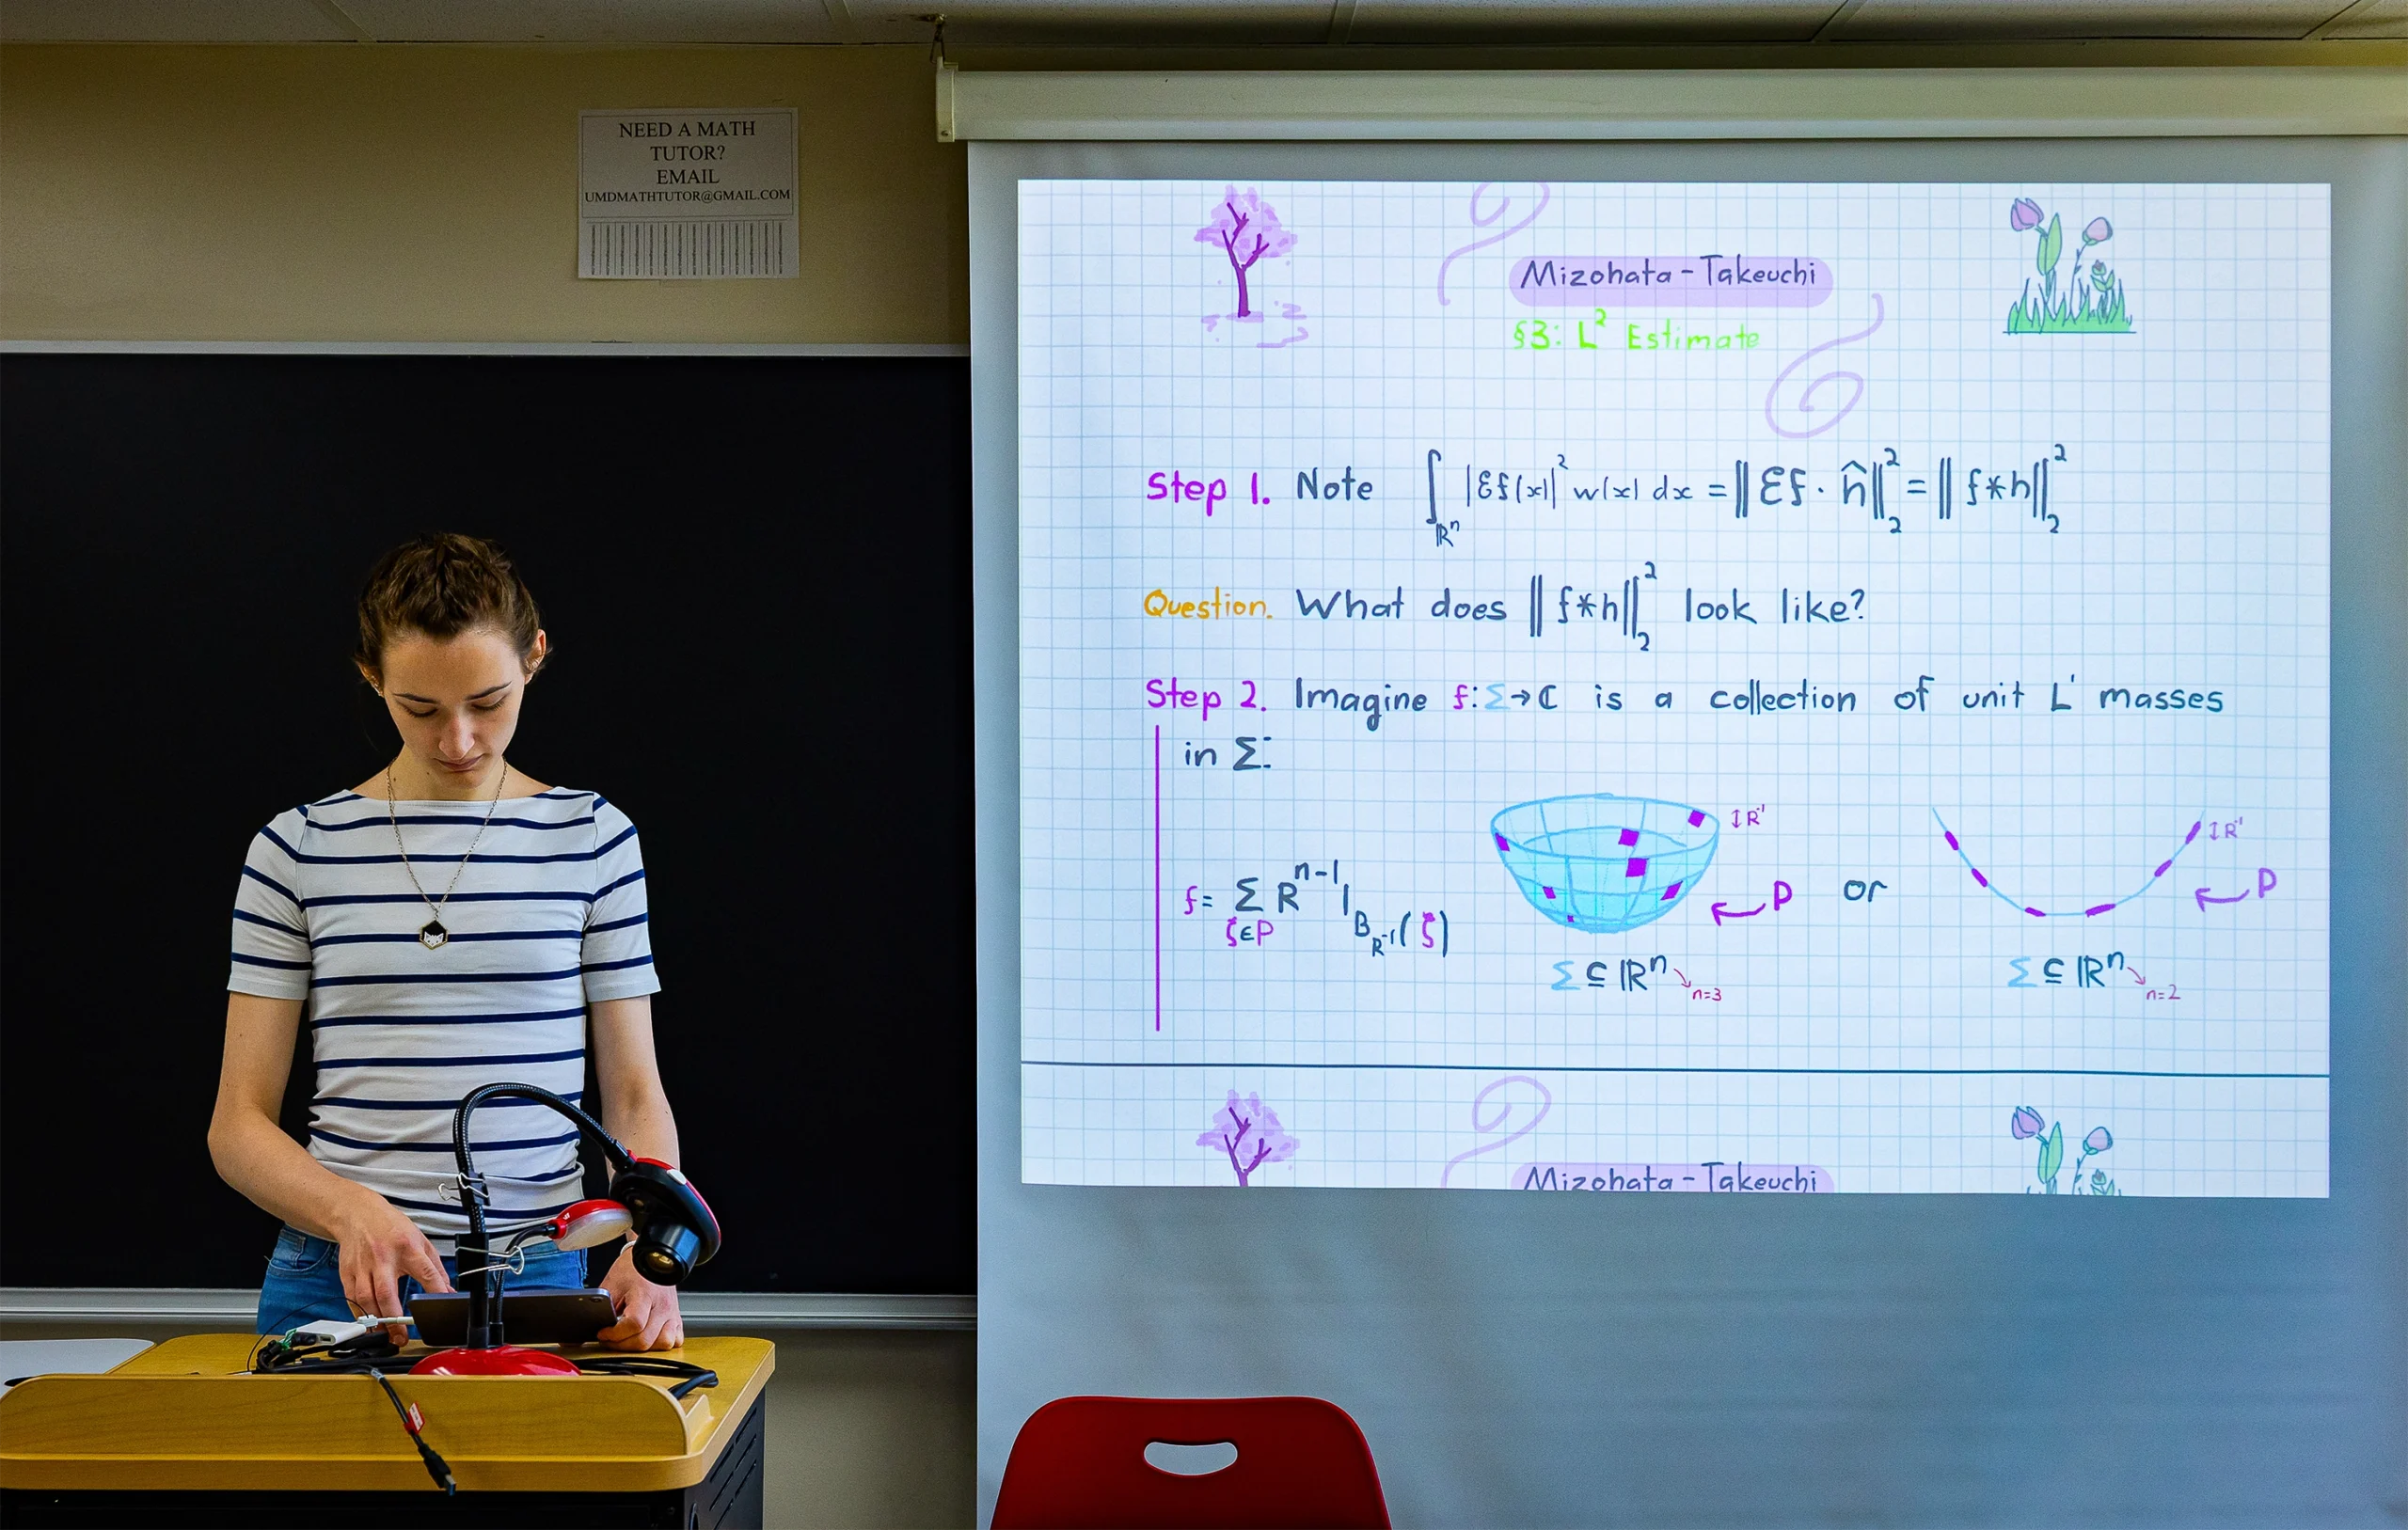
\includegraphics[width =.6\textwidth]{./images_women_in_IT/HannahCairo-cr.ValeriePlesch-Screen-scaled.png} \\
        Mizohata-Takeuchi conjecture\\ Hannah Cairo    
    }
    \only<3>{\includegraphics<3->[width =.6\textwidth]{./images_women_in_IT/Summer_Haag_Clyde_Kertzer.png}\\
            local-global conjecture\\ Summer Haag and Clyde Kertzer
    }
    % \begin{columns}
    %     \begin{column}{.45\textwidth}
    %         % Mizohata-Takeuchi conjecture\\ Hannah Cairo (2008--)
    %     \end{column}
    %     \begin{column}{4.5\textwidth}
    %     \end{column}
    % \end{columns}
\end{frame}

%%Boolean%%%%%%
%%pyramid%%%
\begin{frame}{}
    \begin{columns}
        \begin{column}{.5\textwidth}
        \textbf{\null}%place holder
        \\ \centering \huge 
        \normalsize
            \only<2->{\begin{figure}
                \centering
                \includegraphics[width =.6\textwidth]{./images_5-20-2022/Georg_Cantor_eyes_smile.png}
                \caption*{Georg Cantor (1845-1918)}
            \end{figure}}
            % \only<5->{\begin{figure}
            %     \centering
            %     \vspace{20pt}
            %     \includegraphics[width =.6\textwidth]{./images_5-20-2022/Boole.png}
            %     \caption*{George Boole (1815-1864)}
            % \end{figure}}
        \end{column}
        %%%%
        \begin{column}{.5\textwidth}
            \vspace{10pt}
            \begin{figure}
                \includegraphics<1>[width=.8\textwidth]{./images_5-20-2022/mathpyramid1.png}
                \includegraphics<2>[width=.8\textwidth]{./images_5-20-2022/mathpyramid2.png}
                % \includegraphics<3>[width=.8\textwidth]{./images_5-20-2022/mathpyramid3.png}
                % \includegraphics<4->[width=.8\textwidth]{./images_5-20-2022/mathpyramid4.png}
            \end{figure}
            
        \end{column}
    \end{columns}
\end{frame}


% \usepackage{environ}
% \DeclareMathAlphabet{\mathcal}{OMS}{cmsy}{m}{n}
% \SetMathAlphabet{\mathcal}{bold}{OMS}{cmsy}{b}{n} %for big-O

%\beamerdefaultoverlayspecification{<+->}

% \makeatletter
% \newsavebox{\measure@tikzpicture}
% \NewEnviron{scaletikzpicturetowidth}[1]{%
%   \def\tikz@width{#1}%
%   \def\tikzscale{1}\begin{lrbox}{\measure@tikzpicture}%
%   \BODY
%   \end{lrbox}%
%   \pgfmathparse{#1/\wd\measure@tikzpicture}%
%   \edef\tikzscale{\pgfmathresult}%
%   \BODY
% }
% \makeatother

\tikzset{c/.style={every coordinate/.try,draw=#1!50!white}} %set for coord shift hack
%%%%%%%%%%%%%%%
\tikzset{%
    %%%%keep
    node_style_blank/.style={circle,font=\sffamily\scriptsize\bfseries},
    %%%%%%uncomment to hide labels
    node_styleG/.style={circle, draw=black,fill=black,font=\sffamily\scriptsize\bfseries},
    node_styleB/.style={circle, draw=black,fill=black,font=\sffamily\scriptsize\bfseries},
    node_styleR/.style={circle, draw=black,fill=black,font=\sffamily\scriptsize\bfseries}
    %%%%uncomment to show labels
    % node_styleG/.style={append after command={\pgfextra{\node [right] at (\tikzlastnode.mid east) {\tikzlastnode};}
    %  }, circle, draw=black,fill=black,font=\sffamily\scriptsize\bfseries},
    % node_styleB/.style={append after command={\pgfextra{\node [right] at (\tikzlastnode.mid east) {\tikzlastnode};}
    %  },circle, draw=black,fill=black,font=\sffamily\scriptsize\bfseries},
    % node_styleR/.style={append after command={\pgfextra{\node [right] at (\tikzlastnode.mid east) {\tikzlastnode};}
    %  },circle, draw=black,fill=black,font=\sffamily\scriptsize\bfseries},
}

%%%%%
\begin{frame}{The Art Gallery Problem}
    \begin{figure}
        \centering
        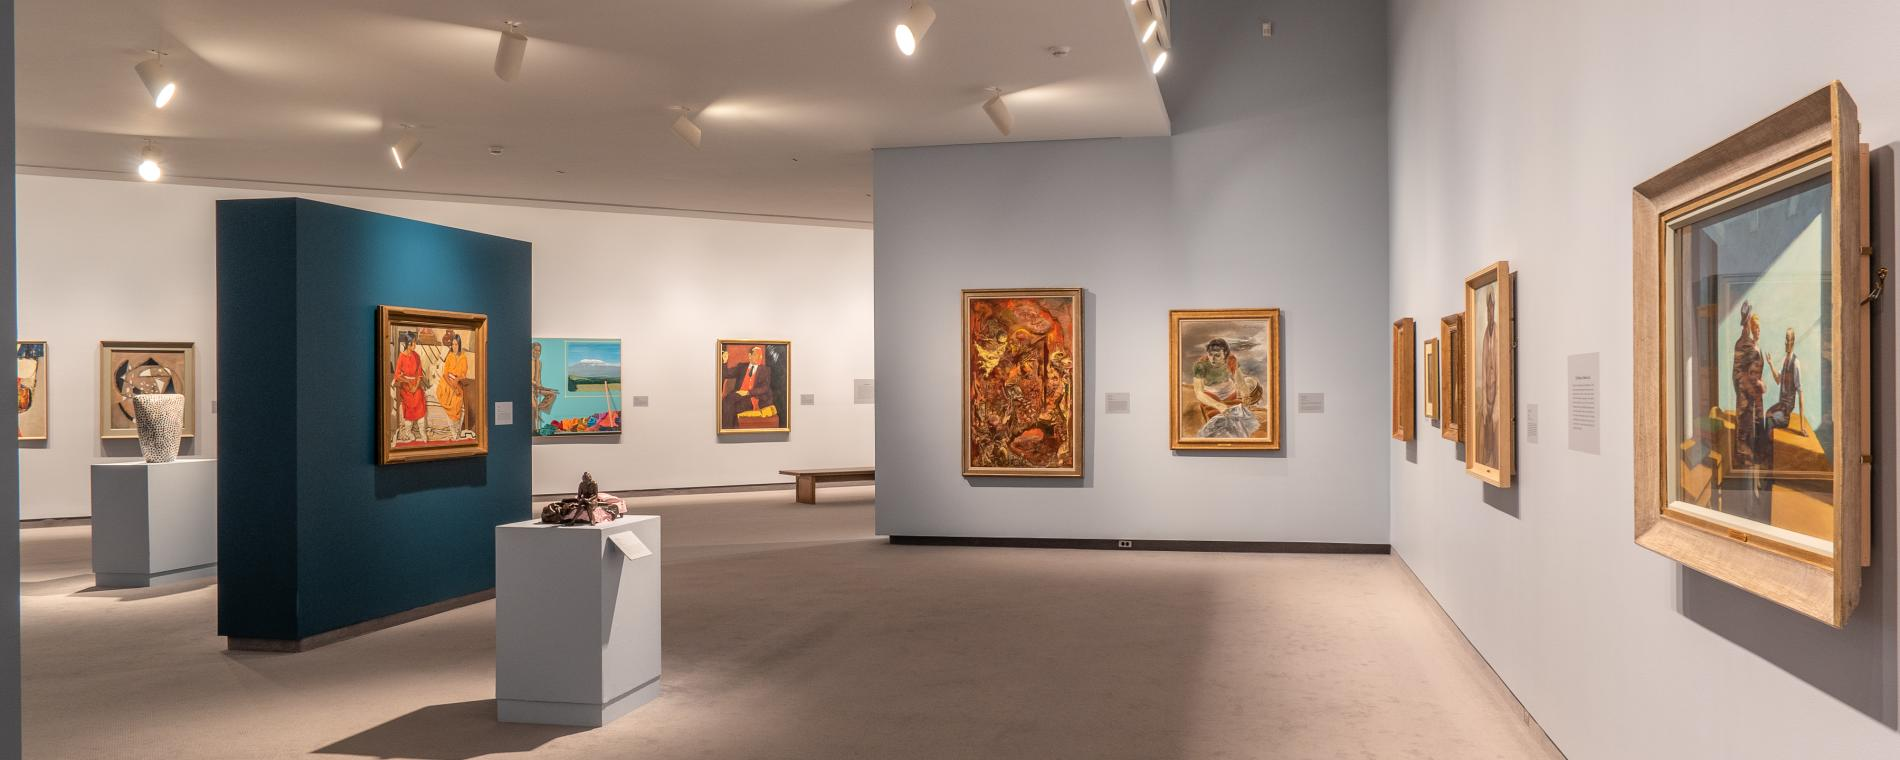
\includegraphics[width=\textwidth]{./images_women_in_IT/Visit_Wichita_Kansas_Wichita_Art_Museum_ab2f81d5-0500-4ccd-af3a-20835143dc89.jpg}
    \end{figure}
\end{frame}

%%%%%
\begin{frame}{How many guards to guard the gallery? Easy case} \label{slide-backstory}
    \def\scalePoly{2}
    \begin{center}
        \only<1>{%
            \begin{tikzpicture}[scale=\scalePoly]
                % create the node
                \node[ultra thick,draw,minimum size=6cm,regular polygon,regular polygon sides=10] (a) {};
                % draw a black dot in each vertex
                \foreach \x in {1,2,...,10}
                  \fill (a.corner \x) circle[radius=2pt];
                % \foreach \x in {2,...,10}
                %   \draw[dashed,<-,red,thick] (a.corner \x) to (a.corner 1);
                % \draw[fill=red] (a.corner 1) circle(.05cm) ;
            \end{tikzpicture}
        }
        \only<2>{%
            \begin{tikzpicture}[scale=\scalePoly]
                % create the node
                \node[ultra thick,draw,minimum size=6cm,regular polygon,regular polygon sides=10] (a) {};
                % draw a black dot in each vertex
                \foreach \x in {1,2,...,10}
                  \fill (a.corner \x) circle[radius=2pt];  
                % \foreach \x in {2,...,10}
                %   \draw[dashed,<-,red,thick] (a.corner \x) to (a.corner 1);
                \draw[fill=red] (a.corner 1) circle(.05cm) ;
            \end{tikzpicture}
        }
        \only<3>{%
            \begin{tikzpicture}[scale=\scalePoly]
                % create the node
                \node[ultra thick,draw,minimum size=6cm,regular polygon,regular polygon sides=10] (a) {};
                % draw a black dot in each vertex
                \foreach \x in {1,2,...,10}
                  \fill (a.corner \x) circle[radius=2pt];
                \foreach \x in {2,...,10}
                  \draw[dashed,<-,red,thick] (a.corner \x) to (a.corner 1);
                \draw[fill=red] (a.corner 1) circle(.05cm) ;
            \end{tikzpicture}
        }
    \end{center}
% No time for that\dots
\end{frame}

%%%%%%%%%%%%%%
\begin{frame}{Most guards needed to guard the gallery? fun case} \label{slide-problem}
        \def\scaleGraph{.65}
        \def\nodeA{\node[node_styleG,] (A) at (-3,4.5) {}}
        % \def\nodeAgreen{\node[node_style, fill = green!50] (A) at (-4,0) {A}}
        \def\nodeB{\node[node_styleB] (B) at (-1.5,2.5) {}}
        \def\nodeC{\node[node_styleG] (C) at (-4.5,1) {}}
        \def\nodeD{\node[node_styleR] (D) at (-2,-4.5) {}}
        % \def\nodeDred{\node[node_style, fill = red!50] (D) at (4,-1) {D}}
        \def\nodeE{\node[node_styleG] (E) at (4.5,-3) {}}
        % \def\nodeEred{\node[node_style, fill =red!50] (E) at (3,3) {E}}
        \def\nodeF{\node[node_styleB] (F) at (4,2) {}}
        \def\nodeG{\node[node_styleR] (G) at (1.5,1) {}}
        \def\nodeH{\node[node_styleB] (H) at (-1.5,-3) {}}
        \def\nodeI{\node[node_styleR] (I) at (-1.5,1) {}}
        \def\nodeJ{\node[node_styleG] (J) at (0.425,0.5) {}}
        \def\nodeK{\node[node_styleR] (K) at (0.5,3.5) {}}
        %%%%
    \begin{center}
    \only<1>{%
        \centering
        \vfill
        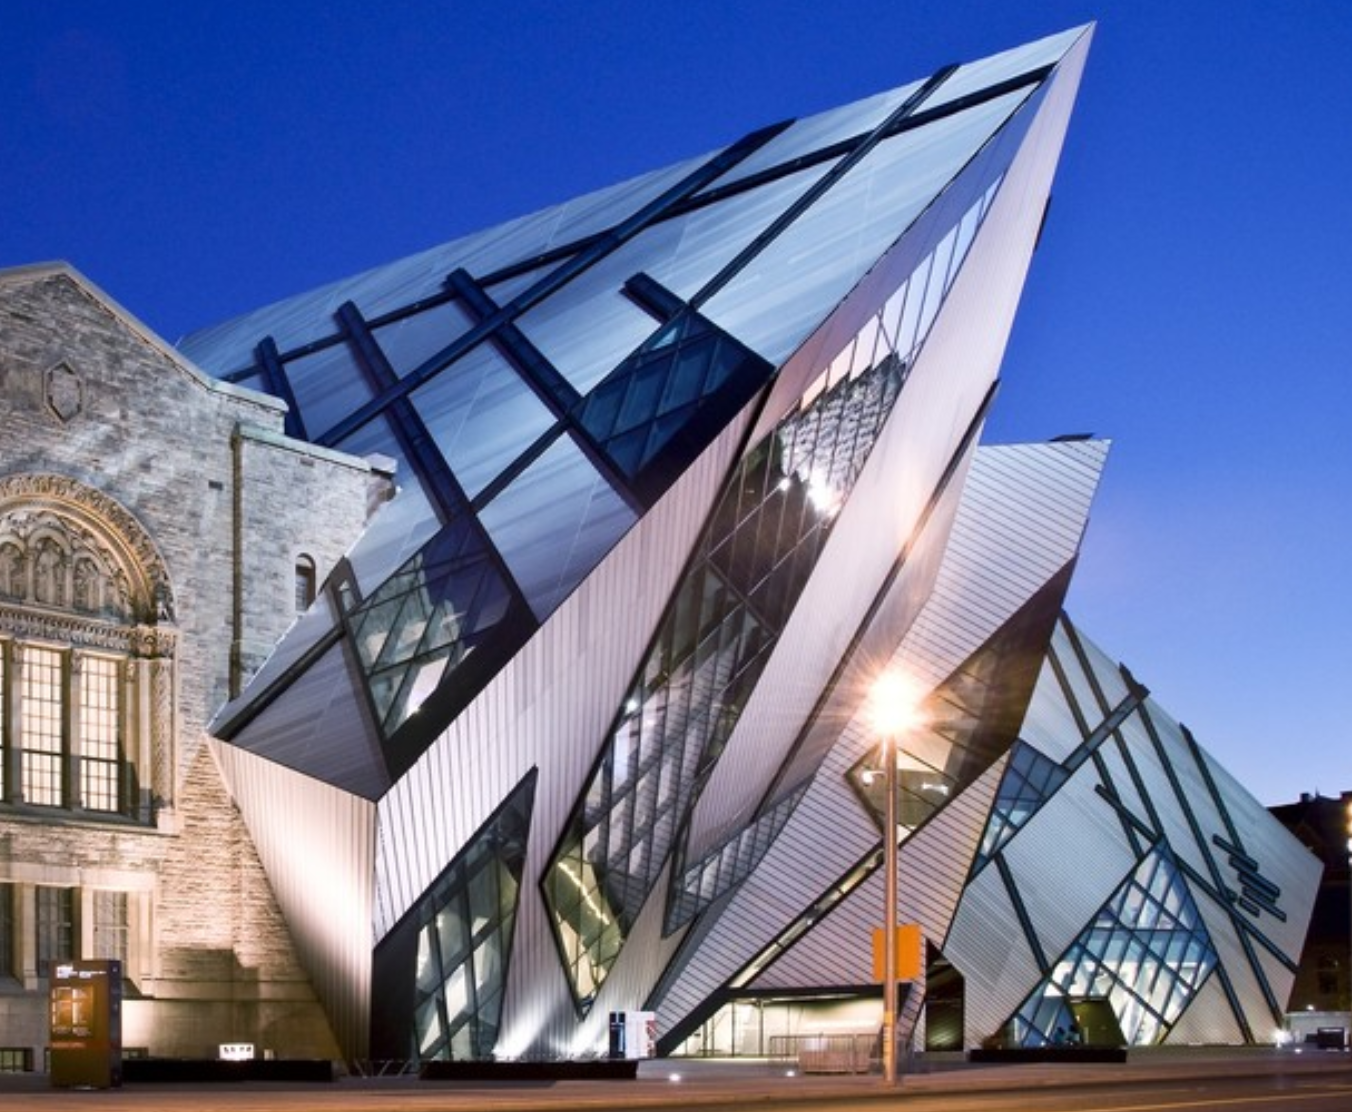
\includegraphics[width=.65\textwidth]{./images_women_in_IT/toronto_art_gallery.png}
    }
    \only<2>{%
        \begin{tikzpicture}[scale=\scaleGraph,shorten >=0pt, auto, node distance=3cm, ultra thick, edge_style/.style={draw=black, ultra thick},label_style/.style={fill=white,text opacity =.5, anchor=center, pos=0.5}] 
            \nodeA;
            \nodeB;
            \nodeC;
            \nodeD;
            \nodeE;
            \nodeF;
            \nodeG;
            \nodeH;
            \nodeI;
            \nodeJ;
            \nodeK;
            \draw[ultra thick,black] (A) -- (B) -- (C) -- (D) -- (E) -- (F) -- (G) -- (H) -- (I) -- (J) -- (K) -- (A);
        % \draw[ultra thick, draw black] (A)-(B)
        \end{tikzpicture}
    }
    \only<3>{%
    Original proof by V.\ Chvital (1975)
    \begin{figure}
        \centering
        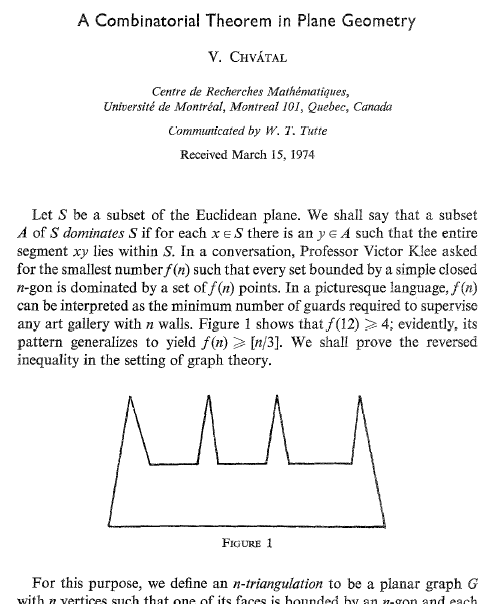
\includegraphics[width=.45\textwidth]{./images_women_in_IT/original_art_gallery_proof-1.png}
    \end{figure}
    }
    \only<4>{%
    Original proof by V.\ Chvital (1975)
    \begin{figure}
        \centering
        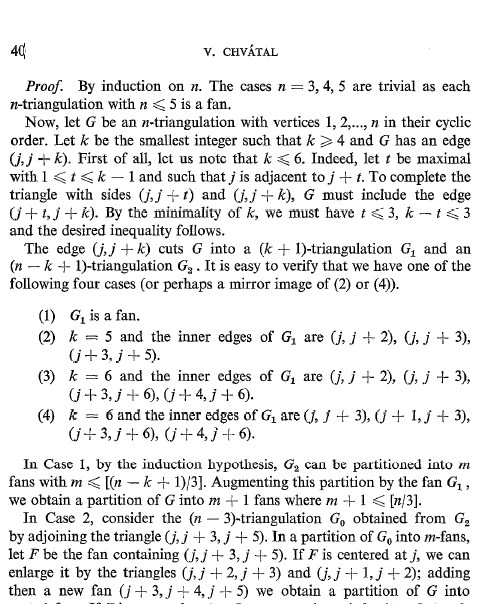
\includegraphics[width=.45\textwidth]{./images_women_in_IT/original_art_gallery_proof-2.png}
    \end{figure}
    }
    \end{center}
\end{frame}

\begin{frame}{}
        \def\scaleGraph{.65}
        \def\nodeA{\node[node_styleG,] (A) at (-3,4.5) {}}
        % \def\nodeAgreen{\node[node_style, fill = green!50] (A) at (-4,0) {A}}
        \def\nodeB{\node[node_styleB] (B) at (-1.5,2.5) {}}
        \def\nodeC{\node[node_styleG] (C) at (-4.5,1) {}}
        \def\nodeD{\node[node_styleR] (D) at (-2,-4.5) {}}
        % \def\nodeDred{\node[node_style, fill = red!50] (D) at (4,-1) {D}}
        \def\nodeE{\node[node_styleG] (E) at (4.5,-3) {}}
        % \def\nodeEred{\node[node_style, fill =red!50] (E) at (3,3) {E}}
        \def\nodeF{\node[node_styleB] (F) at (4,2) {}}
        \def\nodeG{\node[node_styleR] (G) at (1.5,1) {}}
        \def\nodeH{\node[node_styleB] (H) at (-1.5,-3) {}}
        \def\nodeI{\node[node_styleR] (I) at (-1.5,1) {}}
        \def\nodeJ{\node[node_styleG] (J) at (0.425,0.5) {}}
        \def\nodeK{\node[node_styleR] (K) at (0.5,3.5) {}}
        %%%%
        \def\nodeAa{\node[node_style_blank] (Aa) at (-3,4.5) {}}
        \def\nodeBb{\node[node_style_blank] (Bb) at (-1.5,2.5) {}}
        \def\nodeCc{\node[node_style_blank] (Cc) at (-4.5,1) {}}
        \def\nodeDd{\node[node_style_blank] (Dd) at (-2,-4.5) {}}
        \def\nodeEe{\node[node_style_blank] (Ee) at (4.5,-3) {}}
        \def\nodeFf{\node[node_style_blank] (Ff) at (4,2) {}}
        \def\nodeGg{\node[node_style_blank] (Gg) at (1.5,1) {}}
        \def\nodeHh{\node[node_style_blank] (Hh) at (-1.5,-3) {}}
        \def\nodeIi{\node[node_style_blank] (Ii) at (-1.5,1) {}}
        \def\nodeJj{\node[node_style_blank] (Jj) at (0.425,0.5) {}}
        \def\nodeKk{\node[node_style_blank] (Kk) at (0.5,3.5) {}}
        \normalsize
    %%%%%%
    % \only<1>{%
    %     \begin{tikzpicture}[scale=\scaleGraph,shorten >=0pt, auto, node distance=3cm, ultra thick, edge_style/.style={draw=black, ultra thick},label_style/.style={fill=white,text opacity =.5, anchor=center, pos=0.5}] 
    %         \nodeA;
    %         \nodeB;
    %         \nodeC;
    %         \nodeD;
    %         \nodeE;
    %         \nodeF;
    %         \nodeG;
    %         \nodeH;
    %         \nodeI;
    %         \nodeJ;
    %         \nodeK;
    %         \draw[ultra thick,black] (A) -- (B) -- (C) -- (D) -- (E) -- (F) -- (G) -- (H) -- (I) -- (J) -- (K) -- (A);
    %     \end{tikzpicture}
    % }
    %%%%%%
    \begin{columns}[T]
        \begin{column}{.45\textwidth}
            \centering
                \begin{tikzpicture}[scale=\scaleGraph,shorten >=0pt, auto, node distance=3cm, ultra thick, edge_style/.style={draw=black, ultra thick},label_style/.style={fill=white,text opacity =.5, anchor=center, pos=0.5}] 
                    \only<1-3>{%
                        \nodeA; \nodeB; \nodeC; \nodeD; \nodeE; \nodeF; \nodeG; \nodeH; \nodeI; \nodeJ; \nodeK;
                        \draw[ultra thick,black] (A) -- (B) -- (C) -- (D) -- (E) -- (F) 
                        -- (G) -- (H) -- (I) -- (J) -- (K) -- (A);
                    }
                    \only<4>{%
                        \nodeA; \nodeB; \nodeC; \nodeD; \nodeEe; \nodeFf; \nodeGg; \nodeH; \nodeI; \nodeJ; \nodeK;
                        \draw[ultra thick,black] (A) -- (B) -- (C) -- (D) -- (H) -- (I) -- (J) -- (K) -- (A);
                    }
                    \only<5>{%
                        \nodeA; \nodeB; \nodeC; \nodeD; \nodeEe; \nodeFf; \nodeGg; \nodeH; \nodeI; \nodeJ; \nodeK;
                        \draw[ultra thick,black] (A) -- (B) -- (C) -- (D) -- (H) -- (I) -- (J) -- (K) -- (A);
                        \draw[thick,dashed,blue] (K) -- (B);
                        \draw[thick,dashed,blue] (B) -- (J);
                        \draw[thick,dashed,blue] (I) -- (B);
                        \draw[thick,dashed,blue] (I) -- (C);
                        \draw[thick,dashed,blue] (C) -- (H);
                        % \draw[thick,dashed,black] (H) -- (D);
                        % \draw[thick,dashed,black] (H) -- (E);
                        % \draw[thick,dashed,black] (E) -- (G);
                    }
                    \only<6-8>{%
                        \nodeA; \nodeB; \nodeC; \nodeD; \nodeE; \nodeFf; \nodeGg; \nodeH; \nodeI; \nodeJ; \nodeK;
                        \draw<6-7>[ultra thick,black] (A) -- (B) -- (C) -- (D) -- (H) -- (I) -- (J) -- (K) -- (A);
                        \draw[thick,dashed,blue] (K) -- (B);
                        \draw[thick,dashed,blue] (B) -- (J);
                        \draw[thick,dashed,blue] (I) -- (B);
                        \draw[thick,dashed,blue] (I) -- (C);
                        \draw[thick,dashed,blue] (C) -- (H);
                        \draw<7->[thick,black] (H) -- (E);
                        \draw<8->[thick,black] (E) -- (D);
                        \draw<8>[thick,dashed,blue] (H) -- (D);
                        \draw<8>[ultra thick,black] (A) -- (B) -- (C) -- (D) -- (E) -- (H) -- (I) -- (J) -- (K) -- (A);
        
                    }
                    \only<9-10>{%
                        \nodeA; \nodeB; \nodeC; \nodeD; \nodeE; \nodeFf; \nodeGg; \nodeG; \nodeH; \nodeI; \nodeJ; \nodeK;
                        \draw<9>[ultra thick,black] (A) -- (B) -- (C) -- (D) -- (E) -- (H) -- (I) -- (J) -- (K) -- (A);
                        \draw[thick,dashed,blue] (K) -- (B);
                        \draw[thick,dashed,blue] (B) -- (J);
                        \draw[thick,dashed,blue] (I) -- (B);
                        \draw[thick,dashed,blue] (I) -- (C);
                        \draw[thick,dashed,blue] (C) -- (H);
                        \draw[thick,black] (E) -- (D);
                        \draw[thick,dashed,blue] (H) -- (D);
                        \draw<10->[thick,dashed,blue] (H) -- (E);
                        \draw<10>[ultra thick,black] (A) -- (B) -- (C) -- (D) -- (E) -- (G) -- (H) -- (I) -- (J) -- (K) -- (A);
                        % \draw<11>[ultra thick,black] (A) -- (B) -- (C) -- (D) -- (E) -- (F) -- (G) -- (H) -- (I) -- (J) -- (K) -- (A);
                    }
                    \only<11-14>{%
                        \nodeA; \nodeB; \nodeC; \nodeD; \nodeE; \nodeF; \nodeFf; \nodeGg; \nodeG; \nodeF; \nodeH; \nodeI; \nodeJ; \nodeK;
                        \draw<11>[ultra thick,black] (A) -- (B) -- (C) -- (D) -- (E) -- (G) -- (H) -- (I) -- (J) -- (K) -- (A);
                        \draw[thick,dashed,blue] (K) -- (B);
                        \draw[thick,dashed,blue] (B) -- (J);
                        \draw[thick,dashed,blue] (I) -- (B);
                        \draw[thick,dashed,blue] (I) -- (C);
                        \draw[thick,dashed,blue] (C) -- (H);
                        \draw[thick,black] (E) -- (D);
                        \draw[thick,dashed,blue] (H) -- (D);
                        \draw[thick,dashed,blue] (H) -- (E);
                        \draw<12->[ultra thick,black] (A) -- (B) -- (C) -- (D) -- (E) -- (F) -- (G) -- (H) -- (I) -- (J) -- (K) -- (A);
                        \draw<12->[thick,dashed,blue] (G) -- (E);
                        % \draw<12->[thick,dashed,blue] (G) -- (E);
                    }
                    \only<15->{%
                        \nodeA; \nodeB; \nodeCc; \nodeDd; \nodeEe; \nodeFf; \nodeFf; \nodeGg; \nodeHh; \nodeIi; \nodeJj; \nodeK;
                        \draw[ultra thick,black] (A) -- (B) -- (K) -- (A); 
                    } 
                \end{tikzpicture}
        \end{column}
        %%%%%%%
        \begin{column}{.55\textwidth}
            \begin{block}<2->{Claim:}
                Any shape like this can be \textit{triangulated}.
            \end{block} 
            \begin{itemize}
                \item<3->[] IF we can do it for $N$ vertices. 
                \item<8->[] THEN we can do it for $N+1$ vertices. 
                \item[] 
                \item<13->[] So we just need a starting point$\dots$ 
                \item<14->[] $N=3$ 
            \end{itemize}
        \end{column}
    \end{columns}
\end{frame}

\begin{frame}
        \def\scaleGraph{.65}
        \def\nodeA{\node[node_styleG,] (A) at (-3,4.5) {}}
        % \def\nodeAgreen{\node[node_style, fill = green!50] (A) at (-4,0) {A}}
        \def\nodeB{\node[node_styleB] (B) at (-1.5,2.5) {}}
        \def\nodeC{\node[node_styleG] (C) at (-4.5,1) {}}
        \def\nodeD{\node[node_styleR] (D) at (-2,-4.5) {}}
        % \def\nodeDred{\node[node_style, fill = red!50] (D) at (4,-1) {D}}
        \def\nodeE{\node[node_styleG] (E) at (4.5,-3) {}}
        % \def\nodeEred{\node[node_style, fill =red!50] (E) at (3,3) {E}}
        \def\nodeF{\node[node_styleB] (F) at (4,2) {}}
        \def\nodeG{\node[node_styleR] (G) at (1.5,1) {}}
        \def\nodeH{\node[node_styleB] (H) at (-1.5,-3) {}}
        \def\nodeI{\node[node_styleR] (I) at (-1.5,1) {}}
        \def\nodeJ{\node[node_styleG] (J) at (0.425,0.5) {}}
        \def\nodeK{\node[node_styleR] (K) at (0.5,3.5) {}}
        %%%%
        \normalsize
        \begin{columns}[T]
            \begin{column}{.45\textwidth}
                \centering
                \only<1>{%
                    \begin{tikzpicture}[scale=\scaleGraph,shorten >=0pt, auto, node distance=3cm, ultra thick, 
                        edge_style/.style={draw=black, ultra thick},label_style/.style={fill=white,text opacity =.5, anchor=center, pos=0.5}] 
                        \nodeA;
                        \nodeB;
                        \nodeC;
                        \nodeD;
                        \nodeE;
                        \nodeF;
                        \nodeG;
                        \nodeH;
                        \nodeI;
                        \nodeJ;
                        \nodeK;
                        \draw[ultra thick,black] (A) -- (B) -- (C) -- (D) -- (E) -- (F) -- (G) -- (H) -- (I) -- (J) -- (K) -- (A);
                        \draw[thick,dashed,blue] (K) -- (B);
                        \draw[thick,dashed,blue] (B) -- (J);
                        \draw[thick,dashed,blue] (I) -- (B);
                        \draw[thick,dashed,blue] (I) -- (C);
                        \draw[thick,dashed,blue] (C) -- (H);
                        \draw[thick,dashed,blue] (H) -- (D);
                        \draw[thick,dashed,blue] (H) -- (E);
                        \draw[thick,dashed,blue] (E) -- (G);
                        % \draw[ultra thick, draw black] (A)-(B)
                    \end{tikzpicture}
                    }
                \only<2-3>{%
                    \begin{tikzpicture}[scale=\scaleGraph,shorten >=0pt, auto, node distance=3cm, ultra thick,
                    node_styleG/.style={circle,draw=green,fill=green!20!,font=\sffamily\scriptsize\bfseries},
                    node_styleB/.style={circle,draw=blue,fill=blue!20!,font=\sffamily\scriptsize\bfseries},
                    node_styleR/.style={circle,draw=red,fill=red!20!,font=\sffamily\scriptsize\bfseries},
                    node_style_blank/.style={circle,draw=black,fill=black,font=\sffamily\scriptsize\bfseries},
                    edge_style/.style={draw=black, ultra thick},label_style/.style={fill=white,text opacity =.5, anchor=center, pos=0.5}] 
                        \nodeA;
                        \nodeB;
                        \nodeC;
                        \nodeD;
                        \nodeE;
                        % \nodeF;
                        \nodeG;
                        \nodeH;
                        \nodeI;
                        \nodeJ;
                        \nodeK;
                        
                        \draw[ultra thick,black] (A) -- (B) -- (C) -- (D) -- (E) --  (G) -- (H) -- (I) -- (J) -- (K) -- (A);
                        \draw[thick,dashed,black] (K) -- (B);
                        \draw[thick,dashed,black] (B) -- (J);
                        \draw[thick,dashed,black] (I) -- (B);
                        \draw[thick,dashed,black] (I) -- (C);
                        \draw[thick,dashed,black] (C) -- (H);
                        \draw[thick,dashed,black] (H) -- (D);
                        \draw[thick,dashed,black] (H) -- (E);
                        % \draw[thick,dashed,black] (E) -- (G);
                    % \draw[ultra thick, draw black] (A)-(B)
                    \end{tikzpicture}
                }
                \only<4->{%
                    \begin{tikzpicture}[scale=\scaleGraph,shorten >=0pt, auto, node distance=3cm, ultra thick,
                    node_styleG/.style={circle,draw=green,fill=green!20!,font=\sffamily\scriptsize\bfseries},
                    node_styleB/.style={circle,draw=blue,fill=blue!20!,font=\sffamily\scriptsize\bfseries},
                    node_styleR/.style={circle,draw=red,fill=red!20!,font=\sffamily\scriptsize\bfseries},
                    node_style_blank/.style={circle,draw=black,fill=black,font=\sffamily\scriptsize\bfseries},
                    edge_style/.style={draw=black, ultra thick},label_style/.style={fill=white,text opacity =.5, anchor=center, pos=0.5}] 
                        \nodeA;
                        \nodeB;
                        \nodeC;
                        \nodeD;
                        \nodeE;
                        \nodeF;
                        \nodeG;
                        \nodeH;
                        \nodeI;
                        \nodeJ;
                        \nodeK;
                        
                        \draw[ultra thick,black] (A) -- (B) -- (C) -- (D) -- (E) -- (F) -- (G) -- (H) -- (I) -- (J) -- (K) -- (A);
                        \draw[thick,dashed,black] (K) -- (B);
                        \draw[thick,dashed,black] (B) -- (J);
                        \draw[thick,dashed,black] (I) -- (B);
                        \draw[thick,dashed,black] (I) -- (C);
                        \draw[thick,dashed,black] (C) -- (H);
                        \draw[thick,dashed,black] (H) -- (D);
                        \draw[thick,dashed,black] (H) -- (E);
                        \draw[thick,dashed,black] (E) -- (G);
                    % \draw[ultra thick, draw black] (A)-(B)
                    \end{tikzpicture}
                }
        \end{column}
        %%%%%%%
        \begin{column}{.55\textwidth}
            \only<1-4>{%
                \begin{block}<2->{Claim:}
                    Any triangulated shape like can be \textit{tri-colored}.
                \end{block} 
                \begin{itemize}
                    \item<3->[] IF we can do it for $N$ vertices. 
                    \item<4->[] THEN we can do it for $N+1$ vertices. 
                    \item[] 
                    \item<5->[] So we just need a starting point$\dots$ 
                    \item<6->[] $N=3$ 
                \end{itemize}
            }
            \only<5->{%
                \begin{theorem}
                    At most, $\lfloor {\frac{N}{3}} \rfloor$ guards are needed.
                \end{theorem} 
                \begin{itemize}
                    \item<6->[] $\lfloor {\frac{N}{3}} \rfloor$ is just $\frac{N}{3}$ rounded down. 
                    \item<7->[] Since there are $N$ vertices, at least one color will occur $\lfloor {\frac{N}{3}} \rfloor$ times. 
                    \item<8->[] Otherwise the colors would add up to more than $N$. 
                    \item[] 
                    \item<8->[] Post guards at the color! 
                    \item<9->[] In this case \textcolor{blue}{blue}.
                \end{itemize}
                \only<10->{$\frac{11}{3} = 3.666\dots$ so $3$ guards}
            }
        \end{column}
    \end{columns}
\end{frame}

% \begin{frame}
    
%     \uncover<3->{
%         \vspace{-1cm}
        
%         \begin{equation*}
%             \hspace{1cm} \text{At most }\lfloor {\frac{n}{3}} \rfloor \text{ guards.} 
%         \end{equation*}
%         -Fisk's short proof (1978)
%     }
% \end{frame}

%%%%%%%%%%%%%%%
\begin{frame}{} 
\Large
\centering
Proof by Induction
\vspace{10pt}
\large
    \begin{itemize}
        \item<2->[] Assume it's true for $N$.
        \item<3->[] Show it's true for $N+1$ (induction step).
        \item<4->[] Show it's true for any $N$ (base case).
    \end{itemize}
\end{frame}

\begin{frame}{}
    \vspace{10pt}
    \centering
    \begin{figure}
        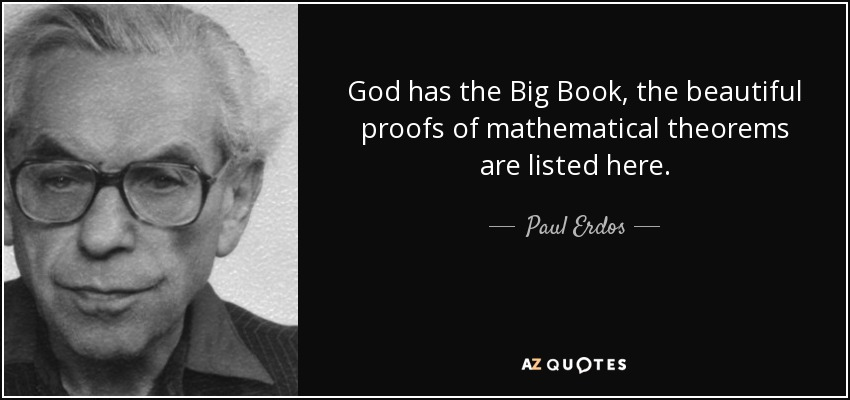
\includegraphics[width=.95\textwidth]{./images_women_in_IT/quote-god-has-the-big-book-the-beautiful-proofs-of-mathematical-theorems-are-listed-here-paul-erdos-35-5-0559.jpg}
    \end{figure} 
\end{frame}

% 
%%True false commands %{
\newcommand{\T}{\textcolor{green!65!black}{\contour{black}{T}}}
\newcommand{\F}{\textcolor{red}{\contour{black}{F}}}
\newcommand{\uT}[2]{\only<#1-#2>{\T}}
\newcommand{\uF}[2]{\only<#1-#2>{\F}}
%}
\begin{frame}{}
    \textbf{Boolean Algebra:} Things are either true or false
    \begin{columns}[c]
        \begin{column}{.4\textwidth}
            % \vspace{-30pt}
            \only<-23>{%
            \begin{itemize}
                \item <2->"I am alive." ($A$)
                \item[] <6-> \hspace{.5cm}\only<6-19>{AND ($\wedge$)} \only<20->{\textbf{OR} ($\vee$)}
                \item <7-> "I am an elephant." ($E$)
            \end{itemize}
            \forestset{  
                	L1/.style={rectangle, rounded corners, shade, top color=white,     bottom color=blue!50!black!20, draw=blue!40!black!60, very     thick},   	
                	L2/.style={rectangle, rounded corners, shade, top color=white,     bottom color=blue!50!black!20, draw=blue!40!black!60, very     thick,
                		edge={black,line width=1.15pt,line cap=round,->}},   	
                	L3/.style={rectangle, rounded corners, shade, top color=white,     bottom color=blue!50!black!20, draw=blue!40!black!60, very     thick,
                		edge={black,line width=1.15pt,line cap=round,->}},   	
                	L4/.style={rectangle, rounded corners, shade, top color=white,     bottom color=blue!50!black!20, draw=blue!40!black!60, very     thick,
                	edge={black,line width=1.15pt,line cap=round,->}}, 
                }
            \uncover<3->{
                \begin{forest} 
            	for tree={
            		scale=.75,        
            		grow=0,
            		reversed, %tree direction         
            		parent anchor=east,
            		child anchor=west, %edge anchors   		edge={line cap=round},
            		outer sep=+1pt, %edge/node connection  		rounded corners,
            		minimum width=15mm,
            		minimum height=8mm, %node shape         l 		sep=10mm %level distance     
            		}   
                    [Start,L1,visible on=<3-> %%for children={visible on=<2->}%%
                    	[\T,L2, visible on=<4->         
                    		[\T,L3,visible on=<9->                     
                    		]         
                    		[\F,L3,visible on=<15->           
                    		]               
                    	]     
                    	[\F,L2,visible on=<5->         
                    		[\T,L3,visible on=<17->                     
                    		]         
                    		[\F,L3,visible on=<18->           
                    		]               
                    	] 
                    ] 
                \end{forest}
            }
        }
            \begin{figure}
                \centering
                \includegraphics<24->[width=.75\textwidth]{./images_5-20-2022/circuit0.png}
            \end{figure}
            \includegraphics<25->[width=.75\textwidth]{./images_5-20-2022/circuit1.png}
        \end{column}
        %%%%
        \begin{column}{.4\textwidth}
            \centering
            \only<8-21>{%
                \begin{tabular}{cc|c}
                     & \multicolumn{1}{c}{} & \tabularnewline
                     & \multicolumn{1}{c}{} & \tabularnewline
                    \textbf{$A$} & \textbf{$E$} & \textbf{$A\only<-20>{\wedge}\only<21>{\vee} E$}\tabularnewline
                    \hline 
                    \uT{8}{} & \uT{9}{} & \uT{10}{}\tabularnewline
                    \uT{15}{} & \uF{15}{} & \uF{16}{20}\uT{21}{}\tabularnewline
                    \uF{8}{} & \uT{17}{} & \uF{17}{20}\uT{21}{}\tabularnewline
                    \uF{18}{} & \uF{18}{} & \uF{19}{}\tabularnewline
                \end{tabular}} 
            \only<22->{
                \begin{tabular}{cc|c}
                     & \multicolumn{1}{c}{} & \tabularnewline
                     & \multicolumn{1}{c}{} & \tabularnewline
                    \textbf{$A$} & \textbf{$E$} & \textbf{$A \vee E$}\tabularnewline
                    \hline 
                    1 & 1 & 1 \tabularnewline
                    1 & 0 & 1 \tabularnewline
                    0 & 1 & 1 \tabularnewline
                    0 & 0 & 0 \tabularnewline
                \end{tabular}
            }
            \\ 
            % \vspace{10pt}
            %venn diagrams
            \begin{figure}
                \centering
            \includegraphics<11>[width=.75\textwidth]{./images_5-20-2022/venn_basic.pdf}
            \includegraphics<12>[width=.75\textwidth]{./images_5-20-2022/venn_A.pdf}
            \includegraphics<13,21>[width=.75\textwidth]{./images_5-20-2022/venn_A_or_B.pdf}
            \includegraphics<14-20>[width=.75\textwidth]{./images_5-20-2022/venn_A_and_B.pdf}
            \includegraphics<23->[width=1.25\textwidth]{./images_5-20-2022/ARM_binary.jpg}
            \end{figure}
        \end{column}
    \end{columns}
    
    \begin{tikzpicture}[remember picture, overlay]
        \node<26> [shift={(0,0)}] at (current page.center) { \includegraphics[scale=0.4]{./images_5-20-2022/Boole.png} };
        \node<27> [shift={(0,0)}] at (current page.center)
        { \includegraphics[scale=0.4]{./images_5-20-2022/BooleCool.png} };
    \end{tikzpicture}
\end{frame}

%%%recap-2%%%
\begin{frame}<9->{D420, D421, D422}
    \begin{columns}
        \begin{column}{.5\textwidth}
            \textbf{D420 \hl<7->{Discrete} Math-Logic}
            \begin{itemize}
                \item \hl<2->{Logic} \& \hl<3->{Proofs}
                \item \hl<9->{Boolean Algebra \& Boolean Functions}
            \end{itemize}
            %%
            \textbf{D421 \hl<7->{Discrete} Math-Functions \& Relations}
            \begin{itemize}
                \item \hl<5->{Set Theory}, \hl<6->{Finite Sequences, \& Series}
                \item \hl<6->{Relations} \& \hl<11->{Directed Graphs}
            \end{itemize}
            % %%
            \textbf{D422 \hl<7->{Discrete} Math-Functions \& Relations}
            \begin{itemize}
                \item \hl<7>{Algorithms}, linear \& associated Big-$\mathcal{O}$
                \item Number Theory \& Cryptography
            \end{itemize}
        \end{column}
        \begin{column}{.5\textwidth}
            \begin{figure}
                \centering
                \includegraphics<3>[width=.5\textwidth]{./images_5-20-2022/proofs.png}
                \includegraphics<4>[width=.5\textwidth]{./images_5-20-2022/proofs.png}
                \includegraphics<5>[width=.5\textwidth]{./images_5-20-2022/sets.png}
                \includegraphics<6>[width=.5\textwidth]{./images_5-20-2022/series.png}
                \includegraphics<7>[width=.65\textwidth]{./images_5-20-2022/discrete.png}
                \includegraphics<8>[width=.65\textwidth]{./images_5-20-2022/cont.png}
                \includegraphics<9>[width=.65\textwidth]{./images_5-20-2022/boolean.png}
                \includegraphics<10>[width=.65\textwidth]{./images_5-20-2022/binary.png}
                \includegraphics<11>[width=.65\textwidth]{./images_5-20-2022/graphs.png}
            \end{figure}
        \end{column}
    \end{columns}
\end{frame}

%%%%RSA alice and bob
\begin{frame}{} %alice and bob RSA
    \centering
    \adjustbox{max width =\textwidth, min height=8cm}{%
    \begin{tikzpicture}[scale=.8]
        % Include the image in a node
        \foreach \n  in {1,...,6}
            \node<\n> [above right,inner sep=0] at (0,0) {\includegraphics[]{./images_5-20-2022/alice_bob_RSA_\n.png}};
        \node<6>[font=\Huge] at (3.15,8.5) {\textbf{?}};
        
        \def\x{5.75}
        \def\y{7}
        \node<7-10> [above right,inner sep=0] at (0,0) {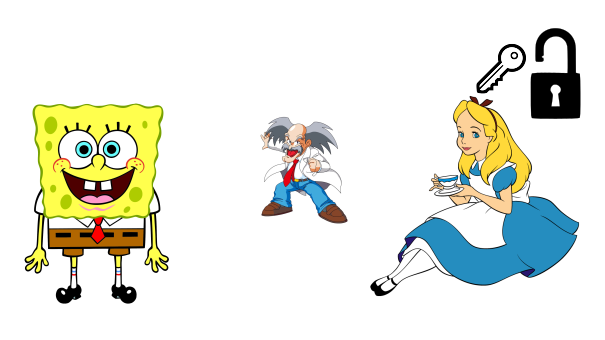
\includegraphics[]{./images_5-20-2022/alice_bob_RSA_7.png}};
            \node<8-10>[rectangle,draw,inner sep =5pt,align=center,font=\Large] at (10,9) {$c\equiv (\text{message})^{e}(\text{mod } N$)}; 
            \node<9-10> [font=\Large,draw, fill=white,align=center] at (10,2.75) {$N = p\times q$ for \textit{secret primes} $p$ \& $q$\\$e$ such that $\gcd(e,(p-1)(q-1)=1$};
            \node<10> [font=\Large,draw, fill=white] at (18.375,8.1) {$N$,$e$};
            
        \node<11-12> [above right,inner sep=0] at (0,0) {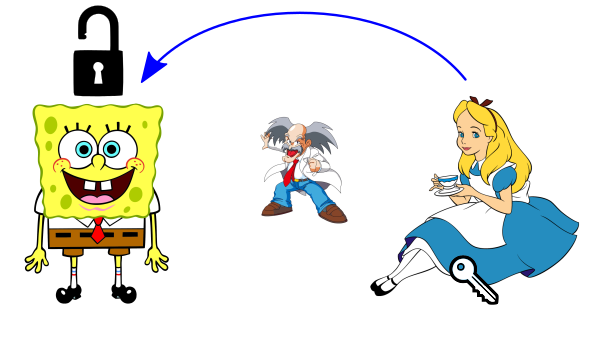
\includegraphics[]{./images_5-20-2022/alice_bob_RSA_9.png}};
            \node<11-12>[font=\Large,draw, fill=white] at (3.25,8.85) {$N$,$e$};
            \node<11-12>[font=\Large,draw, fill=white] at (15.5,2) {$p,q$};
            % \node<12> [font=\Large,right,draw, fill=white,align=center] (a) at (\x,2.75) {$e\times d \equiv 1(\text{mod} (p-1)(q-1))$};
    
    \node<13> [above right,inner sep=0] at (0,0) {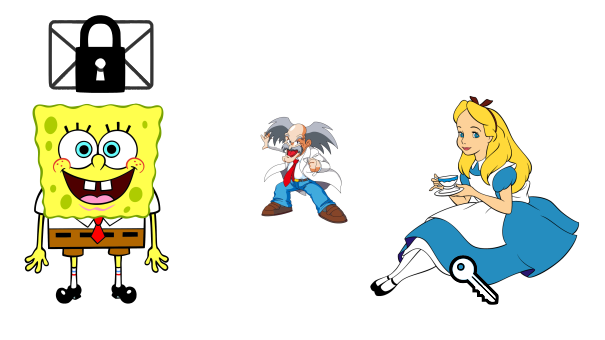
\includegraphics[]{./images_5-20-2022/alice_bob_RSA_10.png}};  
    \node<14> [above right,inner sep=0] at (0,0) {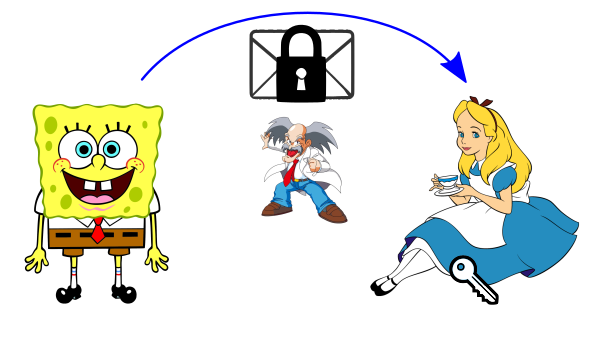
\includegraphics[]{./images_5-20-2022/alice_bob_RSA_11.png}};  
    \node<15> [above right,inner sep=0] at (0,0) {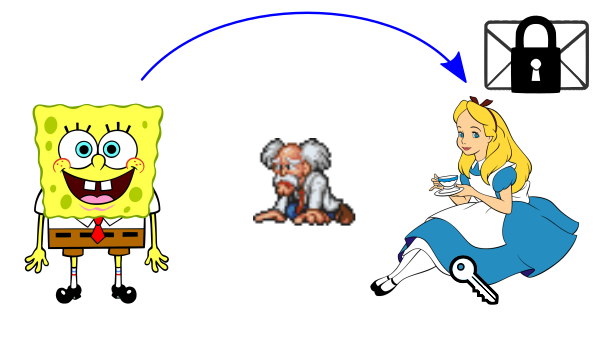
\includegraphics[]{./images_5-20-2022/alice_bob_RSA_12.png}};  
    \node<16-18> [above right,inner sep=0] at (0,0) {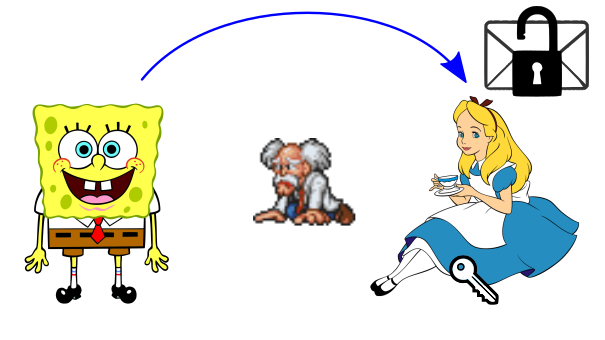
\includegraphics[]{./images_5-20-2022/alice_bob_RSA_13.png}};
        \node<17> [font=\Large,right,draw, fill=white,align=center] (a) at (\x,2.75) {$e\times d \equiv 1(\text{mod} (p-1)(q-1))$};
        \node<17>[font=\Large,draw, fill=white] at (15.5,2) {$p,q$};
        \node<18-19> [font=\Large,right,draw, fill=white,align=center] (a) at (\x,2.75) {$\text{message} \equiv c^{d}(\text{mod} N)$};
    
    \node<19-26> [above right,inner sep=0] at (0,0) {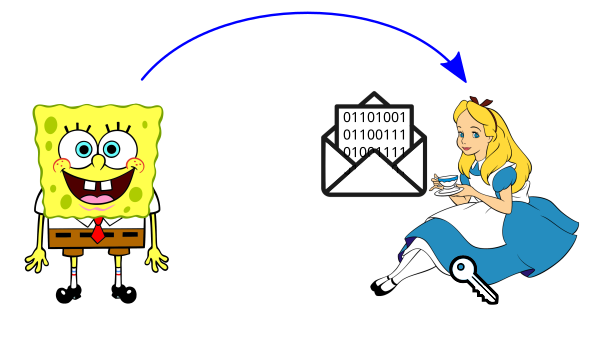
\includegraphics[]{./images_5-20-2022/alice_bob_RSA_14.png}};  
        \node<20-> [font=\Large,right] at (\x,\y) {$\bullet 01101001 \rightarrow$ \textbf{I}};
        \node<21-> [font=\Large,right] at (\x,\y-1) {$\bullet 01100111 \rightarrow$ \textbf{L}};
        \node<22-> [font=\Large,right] at (\x,\y-1.5) {$\bullet 01001111 \rightarrow$ \textbf{O}};
        \node<23-> [font=\Large,right] at (\x,\y-2) {$\bullet 01010110 \rightarrow$ \textbf{V}};
        \node<24-> [font=\Large,right] at (\x,\y-2.5) {$\bullet 01000101 \rightarrow$ \textbf{E}};
        \node<25-> [font=\Large,right] at (\x,\y-3.5) {$\bullet 01111001 \rightarrow$ \textbf{Y}};
        \node<26-> [font=\Large,right] at (\x,\y-4) {$\bullet 01001111 \rightarrow$ \textbf{O}};
        \node<27-> [font=\Large,right] at (\x,\y-4.5) {$\bullet 01010101 \rightarrow$ \textbf{U}};
    \node<27-> [above right,inner sep=0] at (0,0) {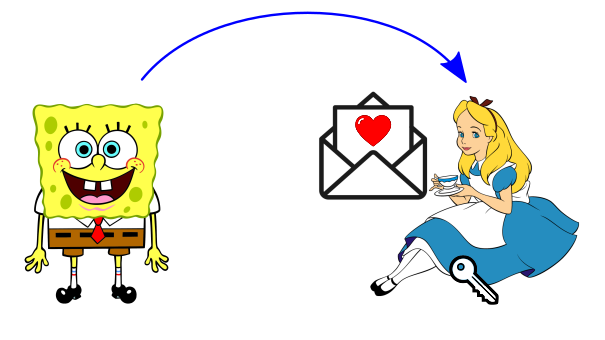
\includegraphics[]{./images_5-20-2022/alice_bob_RSA_15.png}}; 
    %guidelines
        % \draw[above right,help lines,step=1cm,gray!20] (0,0) grid (20,12);
    \end{tikzpicture}
    }
\end{frame}
%%%alice RSA time complexity
%{
\pgfplotsset{%
    axisA/.style = {%
        width=1.0\textwidth,
        % height=.5\textheight,
        % scale=1.0,
        axis lines=middle,
        xticklabels={,,}, yticklabels={,,},
        axis line style={-latex}, 
        ylabel={\footnotesize $f(n)$},             	
        xlabel={\footnotesize $n \rightarrow \infty$},
        x label style={at={(axis description cs:0.5,-0.05)},anchor=north},
        y label style={at={(axis description cs:-0.15,.5)},anchor=south},
        % clip=false, %doesn't clip outside graph
        domain=0:10,
        ymin=0,xmin=0,
        ymax=1000,xmax=25
    },
    axisB/.style = {%
        width=1.0\textwidth,
        % height=.5\textheight,
        % scale=1.0,
        axis lines=middle,
        xticklabels={,,}, yticklabels={,,},
        axis line style={-latex}, 
        ylabel={\footnotesize $f(n)$},             	
        xlabel={\footnotesize $n \rightarrow \infty$},
        x label style={at={(axis description cs:0.5,-0.05)},anchor=north},
        y label style={at={(axis description cs:-0.15,.5)},anchor=south},
        % clip=false, %doesn't clip outside graph
        domain=0:25,
        ymin=0,xmin=0,
        ymax=100,xmax=25
    }
}
\tikzset{
    plotA/.style = {thick, samples=50 
    %  domain=0:18.835
    },
    plotB/.style = {very thick, samples=50, dashed
    %  domain=0:18.835
    }
}
%} 

\begin{frame}{}
    \begin{columns}
        \begin{column}{.4\textwidth}
            \vspace{-6cm} \\
            \only<1-12>{%
                \only<6->{So how hard is it to factor?}
                \only<7->{$\approx 2^{(\text{number's length})}$ steps}
                \begin{itemize}
                    \item<8->[]$3\rightarrow 8$  
                    \item<9->[]$4\rightarrow 16$  
                    \item<10->[]$5\rightarrow 32$  
                    \item<11->[]$\dots$  
                    \item<12->[]$100\rightarrow 1.267\times 10^{30}$  
                \end{itemize}
            }
            \only<13->{%
                \begin{tikzpicture} 
                    \begin{axis}[axisA,plotA,ylabel={\footnotesize $2^{n}$},]
                    	\addplot[red]{2^x} node[above]{};
                    	\only<14>{%
                    	    \node (big-O) at (20,500) {\large \textcolor{red}{$\mathcal{O}(2^{n})$}};
                    	}
                    	\only<15->{%
                    	    \node (big-O) at (18,500) {\Huge \textcolor{red}{$\mathcal{O}(2^{n})$}};
                    	}
                    \end{axis}
                \end{tikzpicture}
            }
        \end{column}
        %%%%%%%%%%%%%%
        \begin{column}{.5\textwidth}
        \adjustbox{max width =\textwidth, min height=8cm}{%
            \begin{tikzpicture}[scale=.8]
            \node [above right,inner sep=0] at (0,0) {
\includegraphics[]{./images_5-20-2022/alice_RSA.png}};  
                \node<2> [font=\Large,draw, fill=white,align=center] at (5,10) {$N = p\times q$ for \textit{secret primes} $p$ \& $q$\\$e$ such that $\gcd(e,(p-1)(q-1)=1$};
                \node<3> [font=\huge,draw, fill=white,align=center] at (5,10) {$N$,$e$};
                \node<4> [font=\Large,draw, fill=white,align=center] at (5,10) {$e\times d \equiv 1(\text{mod} (p-1)(q-1))$};
                \node<5->[font=\huge,draw, fill=white,align=center] at (5,10) {$p,q$};
                % \draw[above right,help lines,step=1cm,gray!20] (0,0) grid (20,12);
        \end{tikzpicture}}
        \end{column}
    \end{columns}
\end{frame}
\end{document}